% The master copy of this demo dissertation is held on Dr. Martin Richards filespace
% on the cl file serve (/homes/mr/teaching/demodissert/)

%% Last Updated by Dorian Peake in 2014

\documentclass[12pt,twoside,notitlepage]{report}

\usepackage{a4}
\usepackage{verbatim}
\usepackage{todonotes}  % todo notes
\usepackage{listings}   % Code listings
\usepackage{color}
\usepackage{graphicx}
\usepackage{amsmath}
\usepackage[utf8]{inputenc}


% set default language to OCaml
\lstset{language=[Objective]Caml,
        basicstyle=\footnotesize\ttfamily,
        keywordstyle=\color{blue},
        numbers=left,
        breaklines=true,
        keepspaces=true,
        frame=single,
        showspaces=false,
        showstringspaces=false
}

%\input{epsf}                            % to allow postscript inclusions
% On thor and CUS read top of file:
%     /opt/TeX/lib/texmf/tex/dvips/epsf.sty
% On CL machines read:
%     /usr/lib/tex/macros/dvips/epsf.tex



\raggedbottom                           % try to avoid widows and orphans
\sloppy
\clubpenalty1000%
\widowpenalty1000%

\addtolength{\oddsidemargin}{6mm}       % adjust margins
\addtolength{\evensidemargin}{-8mm}

\renewcommand{\baselinestretch}{1.1}    % adjust line spacing to make
                                        % more readable
                                        
\usepackage[font={small,it}]{caption}

\begin{document}

\bibliographystyle{plain}
%%%%%%%%%%%%%%%%%%%%%%%%%%%%%%%%%%%%%%%%%%%%%%%%%%%%%%%%%%%%%%%%%%%%%%%%
% Title


\pagestyle{empty}

\hfill{\LARGE \bf Dorian Peake}

\vspace*{60mm}
\begin{center}
\Huge
{\bf Parallelism in OCaml Under the JVM} \\
\vspace*{5mm}
Computer Science Tripos \\
\vspace*{5mm}
St John's College \\
\vspace*{5mm}
\today  % today's date
\end{center}

\cleardoublepage

%%%%%%%%%%%%%%%%%%%%%%%%%%%%%%%%%%%%%%%%%%%%%%%%%%%%%%%%%%%%%%%%%%%%%%%%%%%%%%
% Proforma, table of contents and list of figures

\setcounter{page}{1}
\pagenumbering{roman}
\pagestyle{plain}

\chapter*{Proforma}

{\large
\begin{tabular}{ll}
Name:               & \bf Dorian Peake  \\
College:            & \bf St John's College                     \\
Project Title:      & \bf Parallelism under OCaml using the JVM  \\
Examination:        & \bf Computer Science Tripos, July 2014        \\
Word Count:         & \bf TBC  \\
Project Originator: & Dorian Peake                    \\
Supervisor:         & Jeremy Yallop                   \\ 
\end{tabular}
}
\stepcounter{footnote}


\section*{Original Aims of the Project}

The aim of this project was to highlight the differences between single and multithreaded OCaml code. This was done by adapting the Lightweight Threading Library (LWT) -- a very popular threading library for OCaml -- to use the OCaml
to Java bytecode compiler OCaml-Java, thus allowing software written with LWT to utilise the multithreading capabilities of the JVM.

\section*{Work Completed}
The LWT threading capabilities have been integrated with OCaml-Java via the development of my interface, thus allowing a subset of LWT programs to compile to Java bytecode and run in parallel on the JVM. This is done by scheduling
lightweight threads between Java worker threads which continuously execute code until interrupted. Test code written for this interface achieve similar speedup gains to code written directly in Java (speedup of 3.5 -- 4 with the
interface compared to a speedup of 5 -- 5.5 on normal Java), with an again similar speedup curve -- which is a very positive result. 

\section*{Special Difficulties}
None

\newpage
\section*{Declaration}

I, Dorian Peake of St John's College, being a candidate for Part II of the Computer
Science Tripos, hereby declare
that this dissertation and the work described in it are my own work,
unaided except as may be specified below, and that the dissertation
does not contain material that has already been used to any substantial
extent for a comparable purpose.

\bigskip
\leftline{Signed [signature]}

\medskip
\leftline{Date [date]}

\cleardoublepage

\tableofcontents

\listoffigures

\newpage
\section*{Acknowledgements}
This project was a success thanks to the help of my supervisor Jeremy Yallop, Leo White at the OCaml Labs, Malte Schwarzkopf for his motivation and gift ideas and finally Xavier Clerc for his example code which made developing the
interface a whole lot easier.
%%%%%%%%%%%%%%%%%%%%%%%%%%%%%%%%%%%%%%%%%%%%%%%%%%%%%%%%%%%%%%%%%%%%%%%
% now for the chapters

\cleardoublepage        % just to make sure before the page numbering
                        % is changed

\setcounter{page}{1}
\pagenumbering{arabic}
\pagestyle{headings}

\chapter{Introduction}
\label{chap:Introduction}
\section{Motivation}
\label{sec:motivation}
% What I want to say:
% Talk about how things are moving/have moved from uniprocessor to multiprocessor systems and parallelism. Important to write programs that will run well on the hardware of the day (which means writing programs which exploit
% prarallelism well) and hopefelly will scale easily to hardware of tomorrow.
% Talk about functional programming, what it is, where it came from and why it's good/cool. Examples of C++11 and Java incoroperating functional paradigms, more and more programmers using functional paradigms for type safety(due to
% static typing) efficiency (due to expressiveness of code, first class functions, etc) and abstraction from the complexity of the hardware. Programs written with ML  cannot crash. Mention map-reduce and maybe some other notable
% examlles..
% Security in the mathematics of how it works.
% Talk (more) on OCaml, how it is a 'very good' functional programming language: based on ML, has all the wonderful things I've mentioned about funcitonal programming implemented in the language, incorperates OOP and imerative when
% neccessary but doesn't allow parallelism due to core runtime and non-concurrent garbage collector.
% Enter OCaml-Java, OCaml to java compiler which allows OCaml code to run on the JVM. Also ultimately means that the compiled code can use multiple java threads - now we have truly parallel OCaml code.
% Although OCaml is singlethreaded at the lowest level, there exist threading libraries to perform asynchronous tasks within OCaml, for example Async (developed by Jane Street \citeme} and LWT, produced by Ocsigen). These libraries
% provide a great interface for multithreading in OCaml but lack the underlying support from the OCaml language - It would be interesting to find out just what the benefits and drawbacks exist from executing OCaml asynchrnous code in
% a multithreaded environment (thus the motivation of the project, we can achieve some sort of comparisson between multithreaded and singlethreaded OCaml using OCaml-Java as our vector into multithreaded OCaml code -- Just a matter
% getting one of the asynchronous libraries to work with OCaml-Java.
% How much better is multithreaded OCaml code over singlethreaded code? What are the challenges/benefits of writing multithreaded programs using a functional programming language? How well do threaded/asynchronous OCaml programs
% translate onto a multithreaded system? It would be interesting to test all these things. (possibly only talk about `I wanted to test the difference between using threaded
%
%
% Talk about why multithreading is important
%
Multi-core processors are the focus of chip development in this current day and age. Systems need to continue to increase chip parallelism as this has become the main approach for achieving faster code execution since CPU frequency
speeds plateaued around 2003\cite{hennessy2012}. Of course it is also important for languages and compilers to utilise these advancements in technology, otherwise they will soon become useless for modern software development and
developers will begin to seek more appropriate alternatives that provide them the development resources they need. There also exist software libraries such as OpenCL that are specifically designed to utilise extra computational power
from your GPU which is normally inaccessible for general processing tasks. Clearly parallel processing is a very important topic and is currently a very active research area therefore it is well worth discussion.
\hfill\\
\hfill\\
%
% Talk about why functional programming is important
%
Functional Programming concepts have been around since Turing and Church's work in the 1930's\cite{scott2009} but have become more popular in recent times. The expressiveness that functional programming paradigms give the programmer
has finally caught on in mainstream development and therefore languages such as C++ and Java are incorporating notable functional programming techniques such as type inference\cite{web:autokeyword} and first-class anonymous functions
(lambdas)\cite{web:javalambda}. Notable functional languages include Haskell and ML (which has inspired more widely used functional languages for example OCaml\cite{madhavapeddy2013}). OCaml is a very extensive functional language
which also includes an elegant object system, which incorporates the best of both functional and imperative programming techniques. The ability to develop in these two different programming styles interchangeably makes OCaml a very
powerful language to develop with. Unfortunately OCaml in it's current state is unable to compile parallel code, which of course is becoming an ever more necessary approach to development as systems become more and more
parallel.
\hfill\\
\hfill\\
%
% Talk about how java has multithreading but no functional, whereas OCaml is functional with no multithreading
%
Java is a mature imperative programming language/system widely used in industry to build multithreaded software\cite{web:matlab}. It compiles to Java bytecode which runs on it's virtual machine which in turn is able to run on
everything from ATM's and credit card chips to home desktops and servers -- leading to one of the Java slogans `{\em write once, run everywhere}'. Over the years the JVM has become highly optimised to the hardware/systems that it runs
on such that there is little difference between Java code running on the JVM and natively compiled code. Furthermore, Java supports parallel processing, fully utilising any number of cores/hardware threads that the system has to
offer.
\hfill\\
\hfill\\
%
% Talk about how OCaml-Java merges the two but is in need of a sufficient threading library, many exist (LWT, Async) but are not yet compatible. This is where my project comes in.
%
A project called OCaml-Java aims to merge the best aspects of both OCaml and Java together to create a better OCaml programming solution. It achieves this by compiling OCaml code to Java bytecode, thus allowing it to run on
almost any JVM.
This means two things:
\begin{itemize}
\item OCaml can now be written to run on a wide variety of hardware/systems.
\item OCaml can use Java's multithreading capabilities to run fully parallel OCaml code\cite{clerc2012}.
\end{itemize}
OCaml-Java comes with a basic collection of concurrency tools which are essentially a small subset of Java's own concurrency library with wrappers that allow access from within OCaml. Unfortunately the concurrency techniques provided
by Java do not nicely translate to the way concurrency is done in a functional programming language like OCaml. There do exist commercially-used, optimised OCaml concurrency libraries such as Async by Jane Street and LWT (Lightweight
Threads Library) by Ocsigen, however these do not function when compiled to Java bytecode via OCaml-Java as they rely on the Unix bindings and threads provided either by the OCaml library or similar ones constructed in house.  If we
could get one of these OCaml concurrency libraries to work when compiled with OCaml-Java, we could demonstrate OCaml-Java's true potential to create parallel OCaml code, and OCaml's true capabilities as a parallel programming language
-- this is the motivation for my project. 
\hfill\\
\hfill\\
%
% Briefly outline project, and where I this dissertation will take the reader on their journey
%
My project aims to interface OCaml-Java and the LWT concurrency library in order to demonstrate OCaml's potential as a parallel programming language. The rest of this document outlines the preparation and research I conducted in order
to plan my approach to this project (chapter~\ref{chap:preparation}); the methods and processes that were used to implement the project (chapter~\ref{chap:implementation}) and the result of the project development
(chapter~\ref{chap:evaluation}) and the work process as a whole (chapter~\ref{chap:conclusions}). My code can also be found in appendix~\ref{chap:code_samples}.


% \todo{I don't like the jump between these two paragraphs, seems illogical but they're connected later on}
% Part of the way Programming languages are advancing is towards Functional Programming. Functional Programming concepts have been around since Turing, Church's and Kleene's independent work in the 1930's\cite{scott2009} and
% fundamentally defines the output of a program as the mathematical funcion of its inputs. This is different from imperative languages in that the functions defined in a (purely) functional language have no state and therefore have no
% side effects. If you were to provide the same inputs to the same function you would always get the same output. Another important aspect of functional languages is the idea of functions being first-class values and higher-order
% functions. First-class value functions are functions that are able to be passed as an argument to another function. The function receiving the first-class function argument is known as a higher-order function (which may also return a
% function as a result). Considering these new weapons for development we have obtained from functional programming languages, the expressiveness of our programs has already become incredibly vast. \todo{Might add map function as
% example of higher-order function}.
% Functions such as map, reduce and fold ere very easily expressed using higher-order functions. Java achieves something similar to a higher-order function when using Java Collections, for example Java.util.TreeSet. This class can be
% constructed by passing an object implementing the Comparator interface. This interface contains only one function `compareTo' which creates an ordering between any two elements of a class. Essentially, java is wrapping a class around
% this compareTo function so that it may be passed similarly to a higher-order function. In C you can also pass functions via a function pointer implememnts some aspects of higher-order functions. However bothe Java and C++ are picking
% up many more functional programming paradigms in the latest versions of their languages: Java 8 and C++11\cite{web:javalambda}\cite{web:autokeyword}. Functional programming paradigms are more efficient, with examples such as
% higher-order functions, and safer; many functional languages are almost entirely statically typed which means \todo{no runtime errors, but I'm not sure if thats entirely due to static typing}no runtime errors due to type conflicts and
% faster code (since types do not need to be checked at runtime). The functional programming language ML has become increasingly popular in research institutes and is a great example of a good functional programming
% language. As an example of saftey in functional programming, compiled ML code cannot crash\cite{paulson1996}.


\chapter{Preparation}
\label{chap:preparation}
% Researched into why OCaml cannot fundmentally produce multithreaded code.
% The OCaml-Java paper has a nice section on the reasons that OCaml is not a multithread capable language: Garbage collector is neither parallel nor concurrent and core libraries are not reentrant.
% Ultimately the core libraries can be made reentrant, however sorting out the garbage collector is a more difficult and involved task.
% OCaml does provide a threads library but manual states the threads library is implemented by time sharing on single processor {cite ocaml manual}. 
% Researched into ways of doing concurrent processing in OCaml.
% in conjunction with the OCaml threads library, there are also other threading libraries with a richer feature set, expanding on the OCaml threads library, such as LWT, ASync.
% ultimately the as to which one was solely based on the fact that LWT is more popular, (as I have never worked with either and wouldn't have time to test both of them out and decide which I would like to work with the most).
% Projects exist (such as those given in OCaml-Java paper) on multi-core implementations of ocaml
% Research into LWT
% Lwt is an extensive concurrency suite for OCaml which uses lightweight threads that are created and destroyed very quickly.
% almost all expressions used within LWT results in a thread being created, which returns the answer.
% clearly Java threads and LWT threads are not directly compatible (theres a lot of overhead from creating a Java thread compared to an LWT thread), need some sort of scheduler from LWT threads to Java threads
% describe how LWT works:
%   Lwt.Poll repeatedly checks whether a thread has completed, this is used with Lwt_main.run to start a thread off and relay it's completion to the thread that spawned it.
%   As threads are run, more threads are spawned and put onto the end of a thread queue. In single threaded LWT all the threads are executed in FIFO order (drawing time, draw a thread being taken off, spawning more threads onto the
%   back and then executing the next one on the top of the queue)
% Research into OCaml-Java
% Ocaml-Java provides a `Concurrent' module which provides a few core concurrency solutions e.g. locks, condition variables, atomic variables, etc.
% Also provides a threadign library which allows the creation of Java threads to run bytecode compiled OCaml functions.
% all accessible via OCaml therefore little/no Java will/was needed to link this with LWT. Need to essentially map the functions which are executed in OCaml threads to java threads.
% LWT Threads are lightweight and inexpensive to create/destroy, Java threads are expensive to create/destroy therefore won't be good enough to map each LWT thread to each Java thread.
% Leads to requirements: Maximum java thread lifetime (for efficiency, else parallelism could be drowned out by overheads), and some others...
% Tools used:
% The development of this project relies on the OCaml language, LWT and OCaml-Java
% Used github for backup and version control
% also stored code on dropbox for backup purposes and ease of access

%
% Outline of what is to come in this chapter
%
\hfill\\
This chapter outlines the processes taken in preparation for the project's implementation. I begin with a look into OCaml's multithreaded capabilities, including the limitations around developing parallel OCaml code and why these
limitations exist. I also compare LWT's own asynchronous library in comparison to Java's and the difficulties that may occur when attempting to interface the two. Finally there is an overview of OCaml-Java, including what tools become
available with its use, and its concurrency modules which provide the user with the ability to write parallel OCaml code. 

\section{Investigating Multithreaded OCaml}
\label{sec:investigating_multithreaded_ocaml}
%
% Talk about what makes it impossible to run parallel OCaml code and why OCaml-Java can
%
In order to outline the best implementation plan for the LWT--OCaml-Java interface, it was necessary to understand OCaml's limitations in compiling parallel code. The OCaml-Java paper from the 2012 `Trends in Functional Programming'
collection\cite{clerc2012} states the reason -- the runtime OCaml library is not reentrant and the OCaml garbage collector is neither parallel nor concurrent. Making the runtime library reentrant is a relatively straightforward change
to the system in comparison to making the garbage collector parallel -- which is far more involved -- therefore the real problem is developing a concurrent and parallel garbage collector. Java's G1 garbage collector is fully
parallel\cite{web:garbage-first} and as a result provides multithreaded support of Java applications. Therefore by compiling OCaml code to Java bytecode, the OCaml language may utilise Java's parallelism capabilities.
\hfill\\
\hfill\\
%
% Talk about ways of doing concurrent processing in OCaml
%
It was necessary to decide which of the popular concurrency libraries available to OCaml I should use for the purposes of this project therefore I researched into OCaml's ability to produce concurrent OCaml code. This research led me
to OCaml's own inbuilt threads library. These native threads are designed for single core asynchronous development as the OCaml manual\cite{leroy2013} describes OCaml threads as executing concurrently on a single processor using time
sharing. There exist other concurrency libraries which boast a richer feature set than the one provided by OCaml as default. Examples of these libraries include Async -- developed by Jane Street Capital\footnote{Async Library --
https://github.com/janestreet/async} -- and LWT (Lightweight Threads Library) -- developed by Ocsigen\footnote{Lightweight Threads Library -- https://github.com/ocsigen/lwt}. These are the two main concurrency packages used within
OCaml development, choosing one to use within my project boiled down to which one was most popular. My reasoning is that they are both extremely good packages and would serve well to demonstrate the capabilities of multithreaded
OCaml-Java. LWT won this battle.

\section{Investigating LWT}
\label{sec:investigating_lwt}
%
% Research into LWT, how it works and how it should work in relation to OCaml-Java (i.e. scheduling LWT threads since they're teenie weenie)
%
LWT is an extensive concurrency suite for OCaml which is based around the idea of lightweight cooperative threads\cite{dimino2012} where cooperative threads manage their own life cycle as opposed to preemptive threads which are
controlled externally, e.g. by the operating system. Creating and destroying a thread in LWT are such cheap operations that the system will create a thread for every system call that is executed. This idea of lightweight threads with
a small lifetime is well suited to the way that OCaml (and languages within the ML family) work which is by allocating new immutable data frequently which tend to have very small lifetimes. The OCaml garbage collector is also
optimised for this by using generational garbage collection techniques to more frequently collect younger data since data that has survived a garbage collection once or more before is likely to have an extended
lifetime\cite{chailloux2000}.
\hfill\\
\hfill\\
On the other hand, Java threads have a greater thread creation overhead and as such cannot be used similarly to the way LWT threads are used without detrimental effects to performance. Java's {\tt java.util.concurrent} package avoid
the thread creation overheads by utilising thread pools instead\cite{web:threadpools}. This observation led me to decide that a good implementation strategy for the interface would be to  create a thread scheduler that maps LWT
threads to Java threads as a 1:1 mapping would simply expose great amounts of thread creation overhead, possibly crippling any speedup gains parallelism would obtain.
\hfill\\
\hfill\\
%
% Give some examples of LWT code, how it works, how threads are spawned, joined and bound, the thread queue and how it makes things asynchronous
%
There are many functions within LWT to create threads. One of the most commonly used is the {\tt bind} function, with the following type:
\hfill\\
\begin{lstlisting}
val bind : 'a t -> ('a -> 'b t) -> 'b t
\end{lstlisting}
\hfill\\
The bind function constructs a thread from a thread {\tt t} and a function which takes the return value of {\tt t}. After performing some processing, bind returns a new thread. What this processing does is attach the function as `{\em
waiter}' on the thread. A waiters purpose is to wait until the thread has finished executing, then perform its own execution with the return value of the thread. This serialises the execution of two functions in an asynchronous
environment and acts synonymously to the classic `sync' operation within various writings on parallel processing\cite{cormen2009}. The thread returned by the bind function will contain the final result of the waiter function once
everything has finished executing. Until then, the function thread will remain in the {\tt Sleep} state (moving to the {\tt Return 'a} state once execution has completed). The following listing is an extract from the LWT code base
showing the possible states a thread may exist in:
\hfill\\
\lstinputlisting{thread_state.ml}
\hfill\\
The threads are pretty well commented within the code, however for brevity:
\begin{description}
\item[{\tt Return}]\hfill\\
This state contains the returned value of thread. The return value is the result of the thread completing its execution successfully and terminating.
\item[{\tt Fail}]\hfill\\
The {\tt Fail} state occurs when an uncaught exception is thrown from within the threads execution. The exception is wrapped around this {\tt Fail} variant type so that another thread of execution may determine the appropriate next steps when
dealing with this failed thread.
\item[{\tt Sleep}]\hfill\\
{\tt Sleep} contains the {\tt sleeper} type which holds all the main functionality of a thread. The {\tt waiters} mutable state contains a list of all the functions that will be run when this thread is executed -- it is the execution
body of the thread. There is also state containing data which helps to cancel a thread, etc.
\item[{\tt Repr}]\hfill\\
The {\tt Repr} state just holds the {\tt thread\_repr} type which is actually an indirection of a {\tt thread\_state}. Looking at the {\tt thread\_repr} type we can see that it simply holds another {\tt thread\_state} reference, which
can be any of the above {\tt Return, Fail, Sleep} or {\tt Repr} variants. This allows chains of {\tt thread\_repr} objects pointing to a {\tt Return, Fail} or {\tt Sleep} thread at the end of the chain. This was an interesting problem
to deal with whilst dealing with implementation discussed in \ref{subsubsec:lock_sharing}.
\end{description}
\hfill\\
Since LWT threads are cooperative, there's no real notion of spawning, starting or stopping threads such as in POSIX or Java. Asynchronous execution is achieved by binding some work to a thread which will execute later on. This can be
achieved with the {\tt Lwt\_main.yield} function:
\hfill\\
\begin{lstlisting}
val yield : unit -> unit Lwt.t
\end{lstlisting}
\hfill\\
The {\tt yield} function returns a thread which simply goes to sleep, then wakes up as soon as possible and terminates. This is fairly useless on it's own but binding to this thread will create a situation where you're able to
schedule something as soon as a processor becomes available (which is the point at which the yield thread is woken up).

\section{Investigating OCaml-Java}
\label{sec:investigating_ocaml-java}
%
% Talk about how OCaml-Java achieves concurrency and parallelism (through the concurrency module)
%
OCaml-Java, which provides the framework for compiling parallel OCaml code in this project, is a collection of Java programs and libraries that allow you to compile OCaml code to Java bytecode for execution on the JVM; run OCaml
bytecode compiled software on the JVM using an interpreter written in Java; and access Java libraries directly from within OCaml code using a specially designed interface that maps Java classes to OCaml types. However most relevant
property of OCaml-Java is it's ability to execute OCaml code in parallel using multiple Java threads.
\hfill\\
\hfill\\
%
% Talk about how the concurrency module works, examples of code (maybe, or just prose), how it works (wrapper around java libraries)
%
OCaml-Java provides a concurrency module which contains many standard concurrency features such as locks, atomic variables and condition variables. The locks, for example, can be constructed by calling {\tt make\_reentrant} and
manipulated by calling {\tt lock} and {\tt unlock} to change acquire/release the lock respectively:
\hfill\\
\begin{lstlisting}
val make_reentrant : bool -> t

val lock : t -> unit

val unlock : t -> unit
\end{lstlisting}
\hfill\\
In fact, the concurrency module is just a set of OCaml wrappers around their Java counterparts\cite{web:clerc2013} for example the OCaml-Java reentrant lock module {\tt Concurrent.Lock} is a wrapper around the Java reentrant lock
class {\tt java.util.concurrent.locks.ReentrantLock}.
\hfill\\
\hfill\\
%
% Talk about how OCaml provides neat interface between OCaml and Java with the weird type system (java'lang'system type) etc...
%
For classes that do not yet (and may never) have an OCaml wrapper, there is a neat interface which allows direct calls to Java functions and manipulation of Java references. Via the Java.make and Java.call functions,
you are able to instantiate any Java class or call any Java function. An example which uses this OCaml-Java interface is given below:
\hfill\\
\begin{lstlisting}
let obj = Java.make "java.lang.Object()"
let itg = Java.make "java.lang.Integer(int)" 123l

let obj_hash = Java.call "java.lang.Object.hashCode():int" obj
let eq = Java.call "java.lang.Object.equals(java.lang.Object):boolean" obj itg
\end{lstlisting}
\hfill\\
This code is an example of using the OCaml-Java interface to construct two Java objects named {\tt obj} and {\tt itg} using different classes via the {\tt Java.make} function. Their hash values are compared to each other using {\tt
Java.call} on the {\tt hashCode} method and the {\tt equals} method.  Whilst the Java primitives are easily mapped to OCaml types -- e.g. a Java {\tt int} maps directly to an OCaml {\tt int32} -- the types of Java objects need to have
their own defining types within OCaml in order to cooperate appropriately with the OCaml type system. The typing scheme introduced maps a Java Object to an OCaml type {\tt 'a java\_instance} where {\tt 'a} is a Java class.  Classes
are denoted within OCaml by replacing dots with single quotes to abide by the OCaml syntactic rules\cite{web:clerc2013}, therefore as an example, the equivalent OCaml type for {\tt java.lang.Object} would be {\tt java'lang'Object
java\_instance}.
\hfill\\
\hfill\\

\section{Choice of Tools}
\label{sec:choice_of_tools}
%
% Choice of tools, in this case it is Vim, decided against using Object system of OCaml since LWT doesn't use it at all anyway (stuck to modular for consistency)
% used git for version control and github for code host and backup, also set up a mirror on my PWF facilities. Used dropbox for backup and ease of access
% software engineering techniques involved weekly meetings with supervisors about my progress and my best next step. Working by myself so not neccessary to follow protocols such as Agile Development, but generally had `project days'
% where I would spend the whole day (or two) solely on project work (meaning there was less start-stop overhead from doing bits every day).
%
My project depends entirely on the use of OCaml and Java therefore there is no real decision relating to the programming languages I will use. Furthermore the LWT library and OCaml-Java compiler are two projects that I will be
depending on throughout the development of the project. These invariants aside, the following section outlines my choice of development environment, including version control, backup precautions taken/software used and the development
and build methods applied.

\subsection{Development Environment}
\label{subsec:development_environment}

\subsubsection{Software and Systems}
Unlike Java, OCaml has little in the way of a fully supported integrated development environment (IDE). There are add-ons for IDEs such as Eclipse\footnote{https://www.eclipse.org} which add syntax highlighting and build functions,
however most (including my supervisors) use a text editor such as Emacs or Vim to develop -- which both come stock with OCaml syntax highlighting. I am already very familiar with Vim, therefore it was a clear choice to use it. I also
used Mac OSX as my host operating system as I am a mac user, however, since there are little restrictions to what operating system OCaml (and in particular Java) can run on therefore I was also able to utilise the Intel Labs PWF
machines on occasion which are running Ubuntu.

\subsubsection{Version Control}
For version control I used Git since I'm already familiar with it and furthermore it has always provided me with the necessary tools I need to work effectively and efficiently. I also used Github to host my code on a remote server for
a few reasons:

\begin{itemize}
\item Github provides educational users with free private repositories which I used for this project.
\item Storing my code on a remote server means that I can easily access it from anywhere with internet access, with all my revisions.
\item My supervisors also have accounts on Github meaning they are easily able to check my progress.
\end{itemize}

\subsubsection{Backup}
\label{subsubsec:backup}
In conjunction with Github as my primary backup solution, I also hosted my code on Dropbox in the case I lose work I haven't yet committed. Furthermore I also have mirrors of my Git repository hosted on the PWF facilities which were
pushed to frequently.

\section{Summary}
\label{sec:preparation_summary}
%
% Summary (pretty much a mirror of the introduction to the chapter, tell you what I've just told you)
%
Within this chapter I have described the process of planning and investigation taken in order to prepare for the projects implementation. I have investigated the ways that OCaml and LWT are able to perform asynchronous code
execution, including the cause for OCaml's limitations in fully parallel code compilation and the differences between LWT and Java's handling of threads. Furthermore I have demonstrated the tools that OCaml-Java has introduced which
allow parallel OCaml code to be written and run on the JVM.  Finally I explained that Vim will be my choice of IDE, running on Mac OSX; Git and Github will be used for version control and in addition the PWF facilities and Dropbox
will be used for backup.

\chapter{Implementation}
\label{chap:implementation}
% what did I even do/core parts of the implementation of project:
% benchmarks, including fib, mergesort.
% making LWT functions thread safe (includes attaching locks to threads, ensuring half-baked threads never see the surface)
% Many implementation problems:
%   LWT is a large software solution, incredibly complex and very popular.
%   OCaml-Java is a mature peice of software, never-the-less still has its fair share of bugs.
%   Initially started to try and get LWT to compile (in its entireity) with OCaml-Java, this involved extracting all the build commands from the makefile (via bash -x dump) and manually editing lines with sed & awk to convert it into
%   a format that OCaml-Java could understand (using ocamljava binaries, libraries, manually preprocessing code, etc).
%   OCaml relies heavily on topfind, a software which automatically constructs ocaml compile commands, including all the relevant libraries. Had to remove all the topfind commands and replace them with their generated output,
%   replacing all libraries with the OCaml-Java counterpart.
%   LWT uses a lot of syntactic sugar which is constructed with Camlp4, the OCaml preprocessor. Unfortunately this is currently broken in OCaml-Java, but fortuntely since it's just a preprocessor I managed to manually preprocess the
%   files and replace them inside the code directory (with a little difficulty since Camlp4 reverts to bytecode when the output is redirected to a file, which meant a lot of struggle wondering why the code was being preprocessed to
%   garbage, furthermore the Camlp4 processing is laced throughout the build commands which meant removing all the p4 switches manually)
%   Came accross many bugs in the OCaml-Java during this process:
%       When compiling OCaml code using ocamlc provided by OCaml-Java, the `shebang' isn't included in the bytecode (unlike normal OCaml) therefore you cannot execute it with `./', you must execute it with `ocamlrun'. Caused a lot of
%       pain when trying to figure out why the executeables were not executing.
%       Camlp4 is broken for OCaml-Java 2.0 version 7 and greater. Returns error 'unable to determine class for symbol Camlp4'
%   Managed to get a lot compiling with OCaml-Java, replaced all the C/C++ external calls with exceptions so that I could catch what I needed to implement first to get some kind of result.
%   After getting somewhere close to a compiling LWT, moved onto getting asynchronous I/O working.
%       The greatest difficulty was determining whether a file descriptor in OCaml is the same as a file descriptor in Java and in Unix. The ultimate answer was yes, however Java gives you no access whatsoever to file descriptors of
%       any kind. This means passing file descriptors is either not going to work at all or going to work with a lot of hacking around with Java reflection and JNI.
%   All the problems resulted me having to abandon this section of the project and move onto the parallelism section.

%   refer to thread queuing operation of LWT from preparation section
%   My job was to turn this thread queueing idea into a thread-safe implementation:
%       Started out with creating a worker thread function which will take threads off the thread queue and execute them
%       Whenever Lwt_main.run is called, the worker threads are spawned and continuously process threads on the thread queue until interrupted
%       There is a clear race condition from all worker threads accessing the thread queue simultaneously. To prevent bugs from this, the simple method is to apply a global lock to accessing and processing a thread on the thread
%       queue, keeping parallelism but removing benefits of parallelism (and only introducing overheads).
%       To move away from the global lock, I introduced a single lock around the thread queue which allowed sequential access to the thread list. The lock is released as soon as a thread is removed from the thread queue.
%       The way LWT is written means that threads are incomplete when they're placed onto the yield queue, meaning that a thread may begin executing an incomplete thread.
%       Solution to this problem was to associate a lock with each thread so that only one worker thread may be accessing a thread at a time.
%       When a thread is constructed it is locked initially since it may be incomplete. This is always true for a yield thread since all it does is sleep and re-awaken (which is useless without some waiters hanging on it).
%       Once some waiters have been bound to this yield thread, a callback is run to unlock the thread, allowing a worker thread to now pick it up and begin execution on it.
%       LWT uses a lot of unusual OCaml code for instance the %identity function which allows explicit type casting from any two types.
%           Clearly defeats the point of type safety in OCaml. It is used to destinguish between a thread type `t', wakener type `u' and a thread_repr type.
%           Thread_repr type may be a chain of thread_repr's with the actual thread type at the bottom of the chain - with pointers to any section of the thread.
%           This whole thing is considered one thread and so each level of the chain must share the lock. Furthermore the colapsing function `repr' must manage lock movement correctly.
%   Normal OCaml code uses camlprof to run profiling on OCaml code, however this is not available in OCaml-Java. Meant I needed to write a Profiling module for the benchmarking process.
%   How profiling works:
%       Create a timer object and run Timer.start at the beginning of a function and Timer.stop at the end of a function.
%       Timing results in nanoseconds can be retrieved from Timer.get_nanos, or millis with Timer.get_millis, etc.
%       Simple and fast so as to get an accurate timing between function invocation and return.
%       No other advanced functions neccessary to complete profiling successfully
% laced lwt with locks
% created a small worker thread function which pops off threads from the queue and executes them
% problems occurred because LWT was written in such a way which allthough concurrent, assumes single threaded (and rightfully so, I mean it is OCaml of course)
% this means thread creation is done in parts and a `half-baked' thread can be put on the 

%
% chapter overview, what will I say in this chapter
% talk about requirements you gave in preparation chapter
%

In this chapter, I outline the main directions and considerations taken towards developing the asynchronous framework for LWT on OCaml-Java. These are outlined as follows:
\begin{enumerate}
\item {\em Single Global Lock Approach} \hfill \\
A single global lock is required to be held by any one worker thread (described below) that needs to execute a {\em lightweight thread}. This means that only one worker thread may be executing a lightweight thread at a time -- the other
threads are blocked and waiting on this lock. Whilst this method doesn't fully exploit parallelism, it provides a stepping stone in the process of constructing the worker threads and locking logic required for full parallel processing
in addition to providing an earlier stage to see and record results.
\item {\em Coarse Grained Approach} \hfill \\
This section extends the basic functionality of the runtime lock approach to multiple cores by introducing Java {\em worker threads}. These threads are assigned lightweight threads to work on continuously until the entire program has
completed. Another very important consideration is to ensure that the worker threads are able to cooperate correctly with each other such that each lightweight thread may run in isolation, as if it were running in its native single core,
asynchronous environment. In some ways that LWT is written assume (correctly) that it will be running on a single processor, resulting in the half-baked thread problem outlined below. Therefore I needed to take these assumptions into
account whilst constructing the parallel system.
\item {\em Profiling} \hfill \\
Profiling the performance gains from introducing parallel computation involved choosing appropriate benchmarks and implementing them in an LWT and OCaml-Java compatible manner. Ultimately merge sort and recursive Fibonacci were
implemented to utilise multiple processors, and this section details the design decisions and their functionality within the system.
\end{enumerate}

\section{Parallelism Overview}
\label{sec:parallelism_overview}
%
% Describe how LWT uses thread queue to produce asynchronous requests  
%
The structure that LWT follows in order to create an asynchronous framework ultimately determined what the necessary steps were in implementing the LWT -- OCaml-Java interface. LWT achieves asynchronous execution by storing
yield threads (mentioned in section~\ref{sec:investigating_lwt}) in a queue which will be referred to as the {\em yield queue} from this point onwards. The function {\tt Lwt\_main.run} runs an algorithm which takes an initial
lightweight thread and
continuously polls this passed thread for completion (i.e. the thread state is {\tt Return a} for some {\tt a}). If the lightweight thread has not yet returned a value, the algorithm iterates through the yield queue, executing all the threads contained within it
until it reaches the top of the queue. The algorithm then re-polls the passed thread for completion again, and cycles through the process of executing threads on the yield queue and polling for completion until a value is returned. 

The functions to be executed by the worker threads will most likely add more lightweight threads to the yield queue. These threads are added to the bottom of the queue and are not executed until the next polling iteration.
Figure~\ref{fig:yield_queue} describes the functionality of the yield queue graphically.
\begin{figure}[h!]
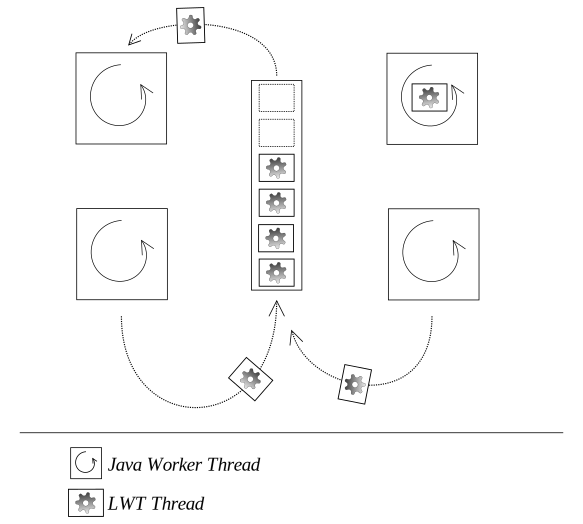
\includegraphics[width=\linewidth]{yield_queue}
\caption[Yield Queue Diagram]{Visual demonstration of the process by which LWT threads are managed and executed on the worker threads. The diagram shows the two bottom worker threads placing LWT threads onto the yield queue, whereas the top left worker
thread is removing an LWT thread from the yield queue and the top right thread is currently processing an LWT thread. Omitted from this diagram is the notion of the yield queue lock which ensures mutually exclusive access to the yield
queue.}
\label{fig:yield_queue}
\end{figure}
%
% Describe how this was translated to run things in parallel with worker threads
%
My approach to creating a parallel model of the yield queue was to mimic the functionality of the {\tt Lwt\_main.run} function across many Java worker threads using OCaml-Java. These worker threads perform the process of
taking threads off the yield queue and executing them. Listing~\ref{lst:worker_thread} summarises the behaviour of a worker thread. Initially the OCaml thread (that is, the first thread executing the main
OCaml code) calls {\tt Lwt\_main.run} with an initial (passed) lightweight thread to execute. This function now spawns multiple worker threads (dependant on the number of physical threads the system has available) which are set
to continually run lightweight threads on the yield queue until interrupted. The OCaml thread begins work on the passed thread which will inevitably spawn other lightweight threads to be pushed onto the yield queue. Once the initial
passed lightweight thread has finished work and is waiting on the spawned lightweight threads to complete, the OCaml thread will continuously poll the passed thread for a return value. Once this return value has been received, the OCaml thread
sends an interrupt signal to all the other worker threads in order to stop processing yield threads and terminate execution.  It is interesting to note that the OCaml thread is governing the other Java threads in a preemptive style
whereas (as mentioned in section~\ref{sec:investigating_lwt}), LWT threads are cooperative -- there were no problems working with the two threading ideas together.
\hfill\\
\lstinputlisting[caption={Worker thread code},label={lst:worker_thread}]{worker.ml}
\hfill\\
%
% Re-describe how yield threads just sleep then wake up. What they execute is whatever is waiting in their waiter list, where a waiter is given by `this datatype'. 
%
As an example, listing~\ref{lst:async_example} is code that when run, simply outputs what thread it is running on. It does this 20 times before quitting, leaving a trace of all the threads that
were executing at that time. The initial lightweight thread passed to {\tt Lwt\_main.run} is executed which spawns a lightweight thread that is placed onto the yield queue, furthermore another function (the waiter function) is bound
to the lightweight thread such that when the thread is awoken and terminates, the function that was bound is then called with the return value of the lightweight thread. This function simply prints out what thread is currently running this
particular code and then adds another lightweight thread to the yield queue, making itself the waiter function. This causes a continuous cycle where lightweight threads are added to the yield queue, taken off by some worker thread, and the name of the worker
thread is printed out. There is a race between the worker threads as to which one picks up the yield thread, therefore the output from running this program may be different each time, demonstrating non-deterministic program
behaviour.
\hfill\\
\lstinputlisting[label={lst:async_example}]{async_example.ml}
\hfill\\
With the overview of the idea for implementing parallel thread execution in LWT, my approach took two main paths: a naive approach of using a single global lock and a coarse grained locking approach. I decided upon these two strategies
because I considered the first approach to be a relatively straight forward way of getting a result from the project whilst also giving insight into potential problems. The second approach was partly based on the concurrency options
that OCaml-Java provided: OCaml-Java provides reentrant locks and semaphores amongst the atomic variables within the concurrency module. Although I had initially decided to use semaphores with integer values based around the
number of threads currently on the queue, as long as there is code running there will be threads on the yield queue because every call in LWT results in a thread. Implementing semaphores would cause more overheads with little
returns, therefore a simple locking scheme was a more sensible idea in this respect.

\subsection{Single Global Lock Approach}
\label{subsec:naive_runtime_lock_apprach}
%
% Discuss implementation that went into the naive runtime lock approach
%
This approach involved having all worker threads require the `global runtime lock' before attempting to pull anything off the yield queue. The lock is also held whilst the lightweight thread is being processed and is only released when all
processing has been finished and the worker thread is about to enter its next iteration of work. All other threads are blocked, waiting on the runtime lock. Although each of the worker threads at this point are running on separate
cores, there is only ever one thread actually running at a time. Furthermore there is now an additional (although minimal) overhead of acquiring the single global lock before execution can proceed. However this approach has created a
foundation for a more efficient method to be implemented.
%
% Maybe a summary of this subsection
%
\subsection{Coarse Grained Locking Approach}
\label{subsec:coarse_grained_locking_apprach}
%
% Discuss implementation that went into the coarse grained locking approach
%
Substituting a single global lock for a coarse grained locking implementation allows the project to take advantage of the parallelism exposed by OCaml-Java. The aim of the coarse grained lock is
to prevent the unnecessary blocking of threads demonstrated in the single global lock approach, by keeping all the worker threads busy via an appropriate scheduler.

%
% Talk about LWT's mutable state and how this lead to a lock per thread
%
Lightweight threads in LWT have mutable state. Consider a lightweight thread state going from {\tt Sleep} with no data to {\tt Return} which lets anything accessing the thread know that the thread has finished executing and has returned its value. It is necessary for
the old {\tt Sleep} thread state to be removed (and collected by the garbage collector) and the {\tt Return} state to be created so the value can be accessed. Therefore the locking mechanism requires that only one worker thread may be
accessing a state at a time to ensure atomic access to the mutable state data. Furthermore, since each lightweight thread may have only one state, the best decision was to associate a lock with each thread
which is to be acquired by all functions that access the thread. 

%
% Talk about solution to thread_refs and lock sharing, including how the repr function collapses the thread_repr's.
%
\subsubsection{Lock Sharing}
\label{subsubsec:lock_sharing}
As briefly mentioned in section~\ref{sec:investigating_lwt}, lightweight threads can have the type {\tt thread\_repr}. This type contains only a reference to another thread which in turn could be a {\tt thread\_repr} type, which results in a
chain of {\tt thread\_repr} objects linking together until some other thread type terminates this chain. At each point in the chain, there may exist some reference to that point from another function or closure,
figure~\ref{fig:thread_repr} depicts an possible {\tt thread\_repr} chain in memory. Although each of these {\tt threadi\_repr} objects are distinct from each other, they all refer to the same base thread object at the bottom of the
chain, whether it be a {\tt Return} or {\tt Sleep}, etc. Therefore it is important to ensure the way the thread locks are used deals with this layering appropriately. In deciding what the best approach for implementing thread locks in
this situation, I came up with the two following methods:

\begin{enumerate}
\item Apply a different lock at each individual level, ensuring all locks are acquired and released at all levels below the current `thread\_repr' level before manipulating the thread data.
\item Have a lock at the lowest level only and ensure this is shared correctly between all other layers.
\end{enumerate}

With method 1, it would be fairly easy to implement the lightweight thread locks as you would simply make a new lock for each {\tt thread\_repr} object, and apply a recursive lock down and throughout the chain. If another worker thread
wishes to use the lightweight thread, they will begin to lock at some point within the chain but then reach a lock which they couldn't acquire. At this point the worker thread could either release its locks and perform some other
useful processing or block on the locked thread.

Method 2 would is also relatively easy to implement but would require sifting through the various LWT ensuring that locks remain connected to their appropriate threads when dealing with mutable state, etc. However sharing the lock
means only one lock operation would need to be performed at any level in the chain which is much more efficient than method 1. For this reason I chose method 2.

\begin{figure}[h!]
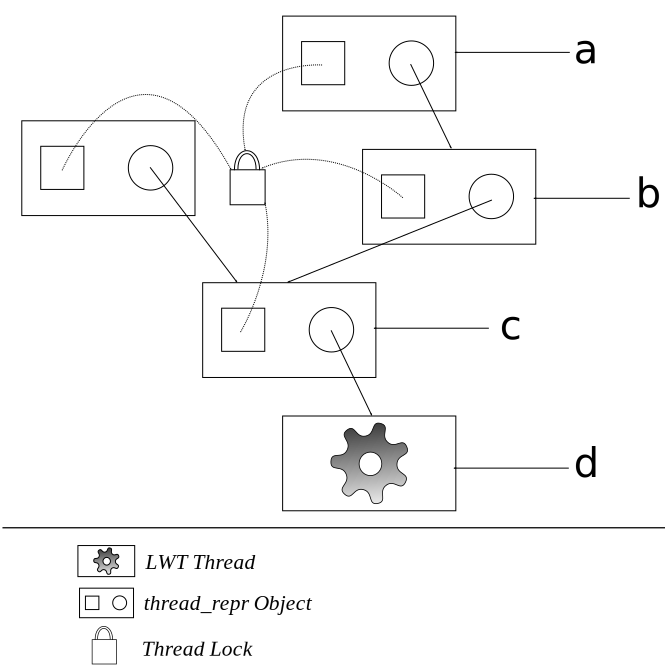
\includegraphics[width=\linewidth]{thread_repr}
\caption[Layered thread\_repr diagram]{The diagram shows an example of an lightweight thread at the bottom of a chain of thread\_repr objects. The letters to the right of each thread\_repr object and the lightweight thread is a reference to the object from within the program. There
may be access at any point within the chain during execution, therefore it is important for every thread\_repr object to share the same lock -- to prevent two worker threads using the same lightweight thread from different points in the
chain. The links between thread\_repr objects always create a directed acyclic graph which is why locking method 1 will always cross a lock which has been acquired if any locks have been.}
\label{fig:thread_repr}
\end{figure}

%
% Other design decisions made/interesing things implemented? take_first_r? no...
%

%
% Summary of the subsection and what it talked about?
%
\subsubsection{Thread Safety}
\label{subsubsec:thread_safety}
%
% Discuss race condition at taking threads off thread queue, easy fix by adding lock around the queue
%

\paragraph{Half-Baked Thread Problem}
\label{para:half-baked_thread_problem}
%
% Discuss race condition at `half-baked' threads being taken off the thread queue (lwt_main.yielded puts it straight on the queue with no waiters, thread run empty, waiters added at end of thread run, thread is garbage collected)
%
Some aspects of how LWT handles threads did not directly map well to a parallel implementation of the interface. In some cases this meant that special care was taken to handle events in an appropriate manner. One notable example
of this is a race condition between lightweight threads being placed on and taken off the yield queue before being appropriately initialised.

A visual description of the problem is outline in figure~\ref{fig:bind_callback}.
\begin{figure}[h!]
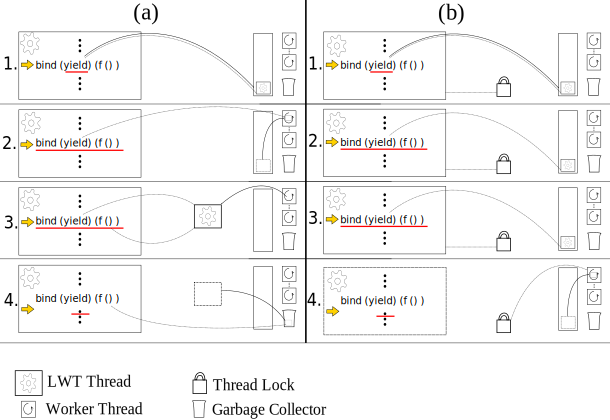
\includegraphics[width=\linewidth]{bind_callback}
\caption[Bind Callback diagram]{Figure (a) describes the process which causes the LWT thread to be exposed before it has finished processing. The dotted arrows represent references still held in memory and the solid lines represent movement of data. 1. The
yield function is called and evaluated to a yield thread. This yield thread is placed straight onto the yield queue. 2. An idle worker thread picks up the yield thread and begins processing it whilst the bind function is processing
more steps. 3. The worker thread has finished executing the yield thread and therefore it remains somewhere in memory. The yield thread is not collected by the garbage collector yet since there is still a reference to the data from
within the bind call. Furthermore since the bind function has not completed at this point, the yield thread execution has not performed anything useful and has just in fact terminated. 4. The bind has now finished attaching a waiter to
the yield thread that should execute when the yield thread is awoken, however this step has already occurred, therefore instead the yield thread is collected by the garbage collector and the function never executes. This is a classic
{\em Time of Check to Time of Use (TOCTTOU)} problem. Figure (b) shows the same 4 steps as figure (a) with the bind callback in place. 1. The yield function is evaluated to a yield thread and the locked yield thread is placed onto the
yield queue. 2. Bind continues to execute but no worker threads are able to acquire the yield thread's lock therefore no worker threads will execute the yield thread. 3. Same as step 2. 4. Bind has finished and the next command begins
executing. Bind has released the yield lock by calling the threads callback function which contains the {\em unlock code}. Now a thread is able to take the yield thread off the yield queue and begin execution with the correct waiters
attached.}

\label{fig:bind_callback}
\end{figure}
The problem occurs when attempting to bind a lightweight thread to a yield thread so that it may be run asynchronously. The yield function adds a thread onto the yield queue instantly without the waiters being added to a waiter list. This means
that any worker thread is able to remove the yield thread from the queue and run it. At the point the bind has added a waiter function to the waiter list, the yield thread has finished executing and will therefore never run the
waiters now attached. Finally the garbage collector picks up the yield thread which has finished and it is never to be seen again. 

%
% Talk about how this was overcome using bind callback
%
Although the section of code where this race condition occurs is relatively small, the problem occurs surprisingly frequently. To overcome this issue, it was necessary to lock the yield thread between the point of creation
and the end of the bind. However this fix makes an assumption on how the yield thread is used -- it suggests that a yield thread will only ever be used in conjunction with a call to bind. While this isn't strictly true, since a yield
thread is a fully qualified lightweight thread on its own that simply does nothing, justification to this assumption is that -- to my understanding -- it is only ever sensibly used in conjunction with bind. To create a yield thread which sleeps
and wakes with no functions to run upon termination is -- useless. Furthermore the only way to achieve some kind of useful processing with a yield thread is to attach a waiter function which will run when the thread terminates.

To lock and unlock the yield thread separated across two functions, I used an additional thread value containing a possibly empty slot for a bind callback. A thread using bind which requires post-bind processing can fill this slot value with
a function that performs the appropriate post-processing. Bind, upon completing its binding operation, will then execute the callback if it exists, finishing off the thread processing appropriately. Using this new bind callback, the
call to yield first locks the yield thread before creation and adds a bind callback function which unlocks the yield thread. In this state, no worker threads will remove a lightweight thread on the yield queue which is currently locked (a requirement
for removing a thread from the yield queue is that the worker thread is able to acquire the thread lock). Once the bind operation has completed on the yield thread, the callback is run which unlocks the thread, allowing it to be
picked up by a worker thread to begin execution.

%
% Special care was taken with the callbacks which could be potentially accessed by many threads simultaneously. Data had to be made atomic, some converted to thread local variables, etc.
%
\paragraph{ACID Callbacks}
\label{para:acid_callbacks}
Callbacks in parallel processing can be called by any and all worker threads that have access to the code and shared data at any time, therefore it was also important to rewrite the LWT callbacks such that each thread accessing the
callback does so in isolation from any other concurrent thread, the shared data is accessed atomically, the shared data remains in a consistent state and the shared data changes remain -- which are the so-called ACID properties of
database transactions. For two out of four of the ACID properties (consistency and durability) LWT's code already manages well, however atomicity and isolation issues needed to be dealt with. This mainly consisted of converting shared
data to their atomic type equivalent, and ensuring data dependencies were kept serialised.

\section{Profiling}
\label{sec:profiling}
%
% Section outline, what this section is about, bla bla bla
%

%
% OCaml normally has camlprof to do profiling of OCaml software, clearly not available in OCaml-Java. Could find a Java profiler however there are many extra functions created when compiling to java bytecode so easier to just write a
% small profiling module
%

%
% Module contains a few timing functions which are direct calls to java.lang.system.gettime (or w.e.) with the timing as the difference between the two returned values (to nanosecond scale). Undocumented how great the overheads are
% for calling java function directly, but they create systematic errors so the speedup scale should remain unchanged (is this correct, i'm sure it is). 
%

Assembling an appropriate profiling suite to test the newly implemented functionality of OCaml-Java and LWT was a step as important as the interface implementation. The regular OCaml compiler allows a special flag for compiling native code with gprof
profiling compatibility\cite{leroy2013}, however this is clearly unavailable since we are compiling to Java bytecode using OCaml-Java. There is no one single Java profiler tool such as gprof, however there are many open source
alternatives. These are highly configurable and complex software suites which allow a lot of configuration -- most of which I wouldn't need. For the purpose of profiling this project, I would simply require an accurate timer to
determine the time taken to complete a function so that these times may be compared and the values used in speedup calculations in chapter~\ref{chap:evaluation}. Taking this into consideration, I wrote a very simple timer module in
OCaml using Java's high-resolution time source via {\tt java.lang.System.nanoTime}. In fact, determining function running time is a typical use of the nanoTime method, as shown by the fact that within the Java documentation example
code is given for exactly that purpose. Listing~\ref{lst:timer} shows some of the commands used within the simple timer module.
\hfill\\
\lstinputlisting[caption={Timer module function types},label={lst:timer}]{timer.mli}
\hfill\\
To utilise Java functions and references directly through OCaml, I used the OCaml-Java interface described in section~\ref{sec:investigating_ocaml-java}. There is no documentation on the speed of executing Java functions via the interface in
comparison to direct calls, therefore it is possible that the interface will introduce some additional overheads, however they did not interfere with the results of the project as demonstrated in chapter~\ref{chap:evaluation}.

%
% Wrote mergesort benchmark (again, example code and how it would run in the system)
%
Choosing an appropriate set of benchmarks which exploits parallelism well was important to demonstrate the true capabilities of my interface. To aid my choice I looked at the Barcelona OpenMP Task Suite and their choices of parallel
benchmarks. One of their benchmarks is an integer sort algorithm based on the Cilk sorting algorithm. The Cilk project is a suite for algorithmic multithreaded programming and the Cilk sort performs a merge sort at the parallel level
and an insertion sort at the sequential level, where sequential sorting is triggered by reaching a sub array size below a particular threshold. Furthermore the classic Introductions to Algorithms book \cite{cormen2009} uses merge sort
as an introduction to parallel algorithms. Therefore the most sensible choice for parallel benchmarking was the parallel merge sort algorithm due to its use in use in professional parallel benchmarking suites and major texts. The merge sort algorithm
I implemented in OCaml is a mirror of the Cilk algorithm with the exception that the insertion sort in Cilk has been replaced with a simple call to OCaml's default array sorting algorithm {\tt Array.sort}.

The merge sort algorithm within the system will continuously add merge sort commands for sub arrays onto the yield queue, where each sub array is half the size of its originating array. This will continue until a sub array
drops below the linear sort threshold, at which point OCaml's default array sorting algorithm is called on the sub array. The threads are taken off the yield queue and executed on multiple worker threads as explained in
section~\ref{sec:parallelism_overview}.

%
% Wrote Fibonacci benchmark (give example code, and talk about how it would run in the system)
%
Another choice of benchmark which was both easy to implement and also featured within the Introduction to Algorithms book was the recursive Fibonacci algorithm adapted for multithreading.

%
% In order to benchmark the speedup gained from parallel OCaml code, I wrote some benchmarks in three different ways: normal OCaml, singlethreaded LWT, parallel/asynchronous LWT.
%

\section{Possible I/O Extensions}
\label{sec:possible_io_extensions}
%
% Describe that attempts were made in Michaelmas/Christmas break on attempting to get entireity of LWT Working
%

%
% Attempt to get LWT to compile and add unimplemented LWT methods afterwards. Came accross a lot of problems...
% A lot of LWT relies on external software which would need to be stripped away or also converted. Tried to get away from build system by dumping all build commands to a build script, then editing manually (using sed, perl)
% Discuss difficulties with using sed on file containing very subtley different commands.
%

%
% Tried to get away from Findlib by replacing Findlib binaries with a `proxy' binary which takes Findlib commands and spits out the OCaml command result.
%

%
% LWT relies heavily on Camlp4. Camlp4 is broken in OCaml-Java and it was a while before I realised it wasn't an error on my part causing difficulties. Managed to use original CamlP4 instead.
%

%
% Managed to strip away all external C/C++ calls and replace then with exceptions so that I could develop the exceptions out one by one
%

%
% Attempting to perform IO between OCaml and Java mean't sharing file descriptors between the representations between the two languages. Unfortunately Java doesn't allow you to tinker with file descriptors at all. Would need to
% perform reflection of sorts to get it working
%

%
% Not much in the way of Documentation for the OCaml-Java -- Java interface, so had to go with a small example provided to my by Xavier Clerc himself.
%

%
% Ultimately time was running short so I had to move on to the actual parallelism by stripping down LWT to it's asynchronous core -- minus any I/O.
%

%
% Learned a lot about taking on a large project. Shouldn't dive straight in, etc...
%
LWT has a very large collection of I/O modules which provide asynchronous I/O functionality and bindings to both Unix and Windows. This set of modules adds a generous amount of functionality to the core asynchronous library
provided by LWT. Now I have converted the core library to work in parallel with OCaml-Java, it is also possible to adapt the LWT I/O modules to also utilise the Java I/O classes to provide asynchronous I/O to the system as
well. 

My approach to this problem would be in three stages:

\begin{enumerate}
\item Attempt to compile LWT in its entirety with OCaml-Java.
\item Filter out external functions that will not run.
\item Build up functionality in stages beginning from the filtered functions.
\end{enumerate}

Attempting to compile LWT in it's entirety is a difficult job in itself as LWT relies on other packages such as OCamlbuild\footnote{OCamlbuild -- http://caml.inria.fr/pub/docs/manual-ocaml-400/manual032.html} and
Findlib\footnote{Findlib -- http://projects.camlcity.org/projects/findlib.html}, which are not fully supported by OCaml-Java. The most straight forward option to compiling LWT would be to manually extract the build
commands from OCamlbuild and output them to a custom build script, which performs the same standard job from a clean build directory. The Findlib package acts as an interface which allows easy package linking and more when building
OCaml programs. Findlib outputs commands which contain all the relevant switches and linked files to compile a piece of OCaml software correctly, therefore by intercepting these commands and replacing them in the build script, I
can remove Findlib and OCamlbuild support entirely. Furthermore LWT also uses the CamlP4 processor to provide many very useful shorthands when writing asynchronous LWT code. However there are a few bugs with the OCaml-Java Camlp4
system, therefore these files can be manually preprocessed using the default Camlp4 preprocessor which will produce the same output.

The second stage involves filtering out foreign function calls that will not run under the JVM. Examples of these commands are calls to system semaphores and mutexes, file manipulation commands and more, as they are all mostly system
dependent. OCaml-Java does not support any foreign function calls written in C/C++, in fact it expects these external command calls to link to Java functions, existing in Java class files. Removing these external function calls from the
OCaml code can be most easily done by replacing the calls with exceptions of the same command name -- done with a sed script. This with both allow the code to compile and also make the third stage of the I/O interface creation process
much simpler.

The third stage involves actually converting the external C/C++ commands into Java code so that it may be executed with (roughly) the same effect as it's C/C++ counterparts. At this stage of the conversion process, the LWT code
should be compiling, however no I/O should yet be working but rather should be terminating with exceptions at the external calls. Depending on what code that I would like to have working first, I would begin with a test LWT program that
utilises I/O, compile it and follow the exceptions, implementing each function until the software executes without fail. The idea is that this would create sections working I/O so that results may be seen sooner than later. An alternative
approach would be to just attempt to implement all the functions, followed by testing and debugging -- however the LWT codebase is large and being unable to test the functions (unable to test easily) would mean there is more code to
sift through during the testing phase. The former approach is far more akin to an iterative/agile development process which is far more flexible to work with.

\section{Summary}
\label{sec:implementation_summary}
In this chapter I began with an overview of how parallelism is achieved between OCaml-Java and LWT, which uses worker threads that are fed lightweight threads off a yield queue, and explained that the rest of the chapter details the
production of this system in it's different approaches. The first approach explained was the single global lock approach which acted mostly as a stepping stone into a stage where LWT was running in parallel on the JVM, whilst abstracting
away the problem thread safety. This was a sensible method of dividing the task of implementing the system as the tasks of attempting to get LWT working on the JVM and exploiting parallelism have minimal overlap. The coarse grained
locking approach section described the transition from parallel poorly scheduled LWT threads, to LWT threads being scheduled appropriately to many simultaneously executing worker threads. This stage introduced thread safety
mechanisms based around lock acquisition and also the unforeseen technical details on getting LWT threads locking across multiple {\tt thread\_repr} objects, and solving the half-baked thread problem. I also ensured all callbacks adhered to the ACID
concurrency properties. Finally the profiling section details the design decisions taken whilst deciding on an appropriate choice of parallel benchmarks to implement for testing purposes, as well as methods of profiling OCaml running
under the JVM without the help of OCaml's default compiler flags and settings.

\chapter{Evaluation}
\label{chap:evaluation}
% Talk about what success critera you've met, and why if any have not been met.
% completed all my success criteria:
%   Able to show scalability difference between 3 versions of benchmarks
%       Need to write/find some program which runs under my software and demonstrates the differences
%   Parallel benchmarks show scalability of LWT running with multithreaded code
%       Clear from the results of the Mergesort graph
% talk how testing was achieved: On my mac, 2 cores 4 hw threads, desktop - similar, roo - 48 core machine.
% implemented fib and merge sort (based on cilk) for parallel benchmarks. Versions written in normal OCaml, LWT and asynchronous LWT to compare the differences between them.
% Graphed number of threads against each other to show speedup
% speedup calculations and other theories e.g. ahmdals law, etc.
% graphed singlethreaded to multithreaded to show scalability
% fib did particularly bad because all it does is expose the overheads of parallelism (one addition per thread, however theres a ton of thread creation and processing behind each one).
% mergesort did much better as when it gets down to 1000 values, the threads are running parallel sorts on 1000 values between 48 cores, which is really fast.
% NEED TO EXPAND ON EVALUATION MORE, THERES LOADS OF GRAPHS I CAN MAKE

%
% Chapter overview, what this chapter talks about, the results acquired, what can be deduced from them, how this relates to your success criteria
%

%
% List success criteria and discuss how each of these were achieved (if at all) also evaluate how the project went
%

Within this chapter I discuss the merge sort test results which are graphed and the nature of the graph shape is explained with a proof that the speedup of parallel merge sort is $O(lg\,n)$, furthermore it is shown that this is
consistent with the results obtained from a parallel merge sort written in Java. We also use the merge sort data do analyse the approximate threading overhead costs to discover how much processing power we are using on thread
management. Fibonacci results are graphed and discussed, including how different implementations of the recursive parallel Fibonacci algorithm can achieve different results. I mention how the tests performed and the results obtained
relate to my success criteria outlined in my project proposal. I also discuss how the tests were run, which consists of a small test suite deployed to the test machines I have been using. 

The following evaluation demonstrates that my success criteria has been achieved. Below is a reminder of these criteria with a small summary of how each criteria has been achieved:

\begin{enumerate}
\item {\em I am able to show the scalability difference between two programs using the same piece of LWT code, one compiled using the original LWT libraries under the normal OCaml compiler and one compiled using my ported LWT libraries
under OCaml-Java, running on the JVM.}\hfill \\
The scalability differences between Fibonacci on normal LWT and my interface are demonstrated within this chapter in section~\ref{sec:fibonacci}.
\item {\em Parallel processing benchmark can be used to determine the scalability using LWT under OCaml-Java and using LWT under the normal OCaml environment.}\hfill \\
The merge sort parallel processing benchmark scalability is also demonstrated in this chapter in section~\ref{sec:merge_sort}.
\end{enumerate}

%
% Talk about how testing was performed. (using Roo and macbook air 2013, specifications given in appendix)
%
\section{Testing}
\label{sec:testing}
To perform the actual testing and result collection, I constructed a small test suite to automate tests both on my own machine and on Roo. Roo is a 48-core computer which I was provided access to by the labs in order to conduct my
experiments. The relevant details of Roo's specifications, along with my own Macbook specifications, can be found in appendix~\ref{apdx:machine_specifications}. This test suite consisted of functions which allow specific test parameters to be passed to the
parallel benchmarks and software, such as the number of Java worker threads that must be created, the size of the merge sort array to be tested and other useful test parameters. The test suite also automatically determines whether
some error occurred during testing by analysing the output and determining whether some tests should be repeated. The analysis does not test for anomalous results but rather incomplete/corrupted results. The help text is shown below:
\begin{lstlisting}[keywordstyle=\color{black}]
Options Are:
    -f      Perform fib tests
    -m      Perform merge sort tests
    -F num  From value
    -T num  To value
    -S num  Step value
    -j num  Number of worker threads to be created in this test 
            (not specifying will cause the test to repeat for 0
             <= j <= cores detected in machine)
    -n num  Size value
    -y num  Type of msort test to do, either msort varying array 
            size (where num = 1) or sort varying linear sort 
            limit (where num = 2). When type 1 is selected, the
            to, from and step values determine the range of 
            array sizes to test (and the step size in-between), 
            where the size value determines the size of the 
            linear sort limit. When type 2 is chosen, the to, 
            from and step values determine the linear sort limit 
            value and the size value determines the array size to 
            be used throughout the tests.
\end{lstlisting}
Without any parameters passed, the test suite simply runs the default tests which provide appropriate numbers for analysis.

\section{Merge Sort}
\label{sec:merge_sort}
The parallel merge sort algorithm briefly mentioned in section~\ref{sec:profiling} provides a good parallelism benchmark to test the interface with. Firstly, each recursive call of the merge sort works on a completely independent sub
section of the array from its sibling's recursive call. This means that (assuming a contiguous in-memory array is used) there is little/no data dependency between concurrent threads running merge sort
and therefore they may run without stalling each other or requiring special locks. Furthermore, the Cilk benchmark which this current merge sort implementation is based on performs a linear sort when the array size drops below a
certain threshold. By adjusting this value appropriately we are able to achieve the best performance gains by allowing LWT threads to perform large chunks of processing and less thread management. The pseudo code for the merge sort
algorithm is provided below:

Don't forget to describe the merge sort algorithm here!\todo{add merge sort pseudo code here}

Apart from the actual sorting algorithm, there is the situation of creating appropriate arrays for the merge sort algorithm to test and sort. In fact the merge sort is provided a random list of numbers from a range equal to the length
of the array: that is, an array of length 10 will contain only the numbers 1 -- 10 at random. This made specifying the range of numbers to the OCaml {\tt Random.int} function easier. Furthermore the merge sort algorithm was to
be run at least twice, once using LWT with no parallelism and one with parallelism, therefore I made copies of the arrays and provided the copies to each function so that they would work on the same, equal data. However the array's
do change between different instantiations of the test, such as when changing the number of worker threads being tested.

\subsection{Performance Analysis}
\subsubsection{Merge Sort Speedup}
\label{subsec:merge_sort_performance_analysis}
The performance results of the merge sort algorithm are shown in the speedup graph in figure~\ref{fig:msort_speedup_graph}, where the x~axis gives the number of cores in use and the y~axis is the speedup, calculated as
$T_1 / T_n$ where $T_1$ is the time taken to perform the sort on 1 thread and $T_n$ is the time taken to execute the sort on n threads.
\begin{figure}[h!]
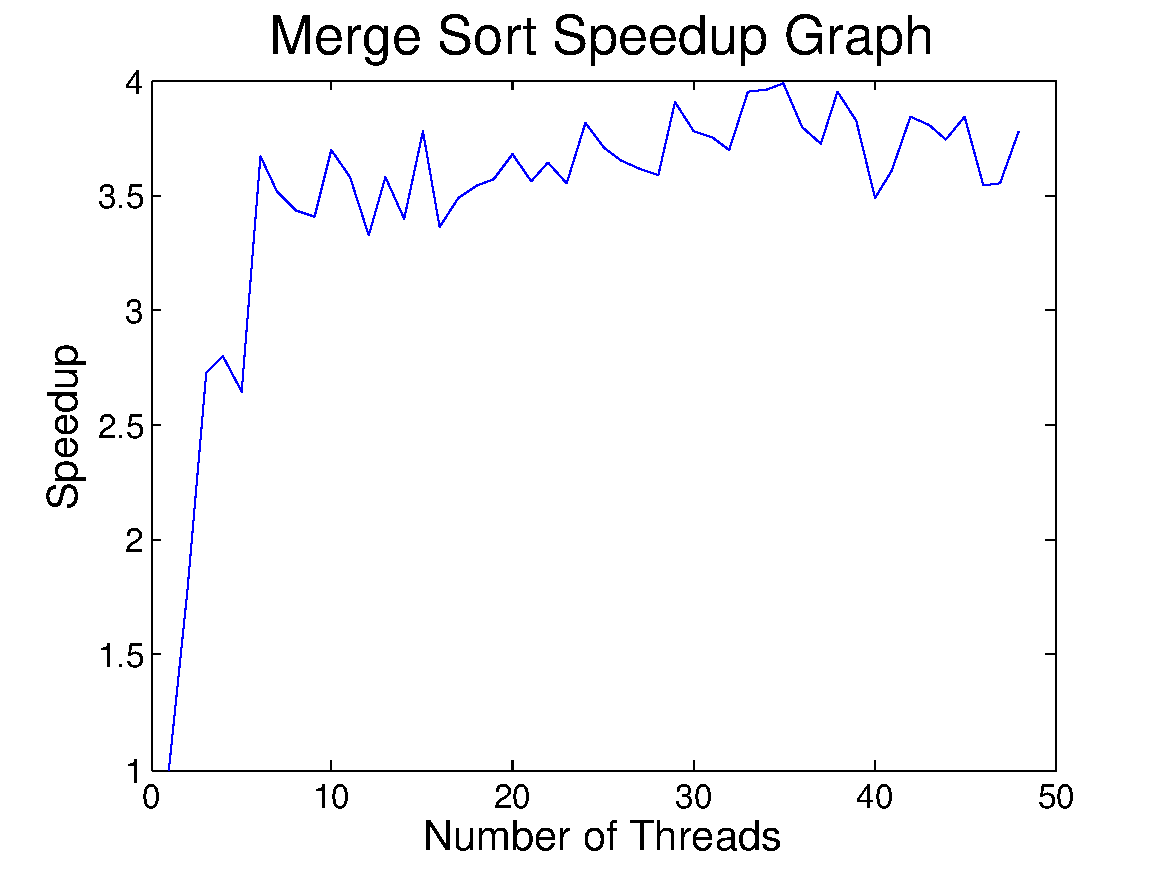
\includegraphics[width=\linewidth]{msort_speedup_graph}
\caption[Parallel Merge Sort Speedup Graph]{The merge sort speedup graph, plotted with a range between 1 and 48 cores on the x~axis; speedup calculated as $T_{1} \over T_{\infty}$ along the y~axis. The graph shows a logarithmic curve which seems to plateau around 3.5
-- 4 times speedup. The logarithmic shape is exactly what should be expected as the merge sort algorithm has maximum speedup in the order $\Theta(lg\,n)$ which is shown within section~\ref{subsec:merge_sort_performance_analysis}.
This result is also mirrored in a normal Java merge sort speedup graph shown in figure~\ref{fig:java_speedup_graph}. Interesting aspects of the graph are the jitter, which can be explained by the fact that the asynchronous nature of
the algorithm means that the execution paths are slightly different each time, in conjunction with the fact that the arrays are generated randomly each time with only similar length therefore the array ordering may cause a faster or
slower execution time.}
\label{fig:msort_speedup_graph}
\end{figure}
There is a clear, almost linear speedup between using 1 and 8 cores for the sort, reaching up to a maximum speedup of between approximately 3 or 4. However after this point, the graph seems to plateau with a little jitter in between
successive increments in the number of cores.

We can first analyse the serial and parallel merge sort algorithms mathematically and then apply this to the outcome of the graph. It is a well known fact that the average running time of merge sort is $\Theta(lg\,{n})$, this can be
shown by considering the following recurrence relation:

\[
T(n) = 
    \begin{cases}
    2T\left({n \over 2}\right) + \Theta(n) & \text{if } n > 1 \\
    1 & \text{if } n = 1
    \end{cases}
\]

This recurrence relation is constructed by dividing the merge sort into its component operations: {\em Divide, Conquer and Combine}\footnote{Divide, Conquer and Combine is the way CLRS describes the separate stages of merge sort. I
believe this is very clear and sensible and therefore have done the same here}:

\begin{description}

\item[Divide] \hfill \\
The dividing process simply splits the array into two smaller sub arrays. This is a cheap operation since all that is needed is to calculate the existing address of the sub array in memory.

\item[Conquer] \hfill \\
Conquering consists of performing a recursive call on the two sub arrays created in the divide process. If the time taken to perform a merge sort on an array of size $n$ was $T(n)$ then the conquer process must perform this operation
twice on two sub arrays of half the size, resulting in the term $2T({n \over 2})$.

\item[Combine] \hfill \\
The combining phase is the {\em merge} of the merge sort algorithm, which runs linearly through the two arrays, creating a larger merged and sorted array, in time $\Theta(n)$ for sub arrays of size $n$ each.

\end{description}

Solving this recurrence relation is relatively simple algebra with a little substitution:
\begin{align*}
T(n) &= 2T\left({n \over 2}\right) + \Theta(n) \\
&= 2\left(2T\left({n \over 4}\right) + \Theta\left({n \over 2}\right)\right) + \Theta(n) \\
&= 4T\left({n \over 4}\right) + 2\Theta(n) \\
&= 8T\left({n \over 8}\right) + 3\Theta(n) \\
\end{align*}

At this point if we let $n = 2^{m}$ we get:

\begin{align*}
&= 2^{3}T\left(2^{m-3}\right) + 3\Theta\left(2^{m}\right) \\
&= 2^{k}T\left(2^{m-k}\right) + k\Theta\left(2^{m}\right) & \forall k \geq 0\\
\end{align*}

Letting k tend to m (approaching the smallest sub array size):

\begin{align*}
&= 2^{m}T\left(2^{0}\right) + m\Theta\left(2^{m}\right) \\
&= 2^{m} + m\Theta\left(2^{m}\right) \\
&= n + lg(n)\Theta(n) & \text{substituting $2^{m}$ for $n$} \\
&= \Theta(n\,{lg\,{n}}) 
\end{align*}

This is the average running time of a serial merge sort and also the work of a parallel merge sort (where work is denoted $T_1$), therefore this value is the running time it should take a merge sort to complete on a single core. Given
the opportunity to utilise many cores, there are subtle changes to the occurrence relation. For my current implementation of merge sort, the merge operation still remains linear, therefore this term remains as $\Theta(n)$, however the
recursive call is able to run on different cores simultaneously, therefore this term now becomes $T'({n \over 2})$ where $T'$ is the parallel merge sort time. Thus the recurrence relation looks like:

\begin{align*}
T'(n) &= T'\left({n \over 2}\right) + \Theta(n) \\
&= T'\left({n \over 4}\right) + \Theta\left({n \over 2}\right) + \Theta(n) \\
&= T'\left({n \over 8}\right) + \Theta\left({n \over 4}\right) + \Theta\left({n \over 2}\right) + \Theta(n) \\
\end{align*}

Similar to last time, let $n = 2^{m}$:

\begin{align*}
&= T'\left(2^{m-3}\right) + \Theta\left(2^{m-2}\right) + \Theta\left(2^{m-1}\right) + \Theta(2^{m}) \\
&= T'\left(2^{m-k}\right) + \sum_{r=0}^{k-1} \Theta\left(2^{m-r}\right) & \forall k \geq 0 \\
\end{align*}

Let k tend to m:

\begin{align*}
&= T'\left(2^{0}\right) + \Theta\left(2^{1}\right) + \ldots + \Theta\left(2^{m}\right) \\
&= 1 + \Theta\left(2^{1} + 2^{2} + \ldots + 2^{m}\right) \\
&= \Theta\left(2^{m+1} - 1\right) \\
&= \Theta\left(2\cdot2^{m}\right)
= \Theta\left(2n\right)
= \Theta\left(n\right)
\end{align*}

Taking into consideration the ability to run the recursive calls on many processors, we have calculated the parallel merge sort average running time, which is also the span of a parallel merge sort (span denoted by $T_\infty$). So
currently we have the results $T = T_{1} = \Theta(n\,lg\,n)$ and $T' = T_{\infty} = \Theta(n)$, for which we can use to calculate the theoretical speedup between serial and parallel merge sort:

\begin{align*}
\text{Speedup} = {T_{1} \over T_{\infty}} = {\Theta\left(n\,lg\,n\right) \over \Theta(n)} = \Theta(lg\,n)
\end{align*}

Therefore in fact we are expecting to see a logarithmic shaped graph as our speedup graph, which is exactly what figure~\ref{fig:msort_speedup_graph} shows us. Figure~\ref{fig:java_speedup_graph} shows a parallel merge sort written
in Java\cite{web:washington} with the same test parameters and the speedup results obtained from these tests which mirrors the results obtained from using the interface.
\begin{figure}[h!]
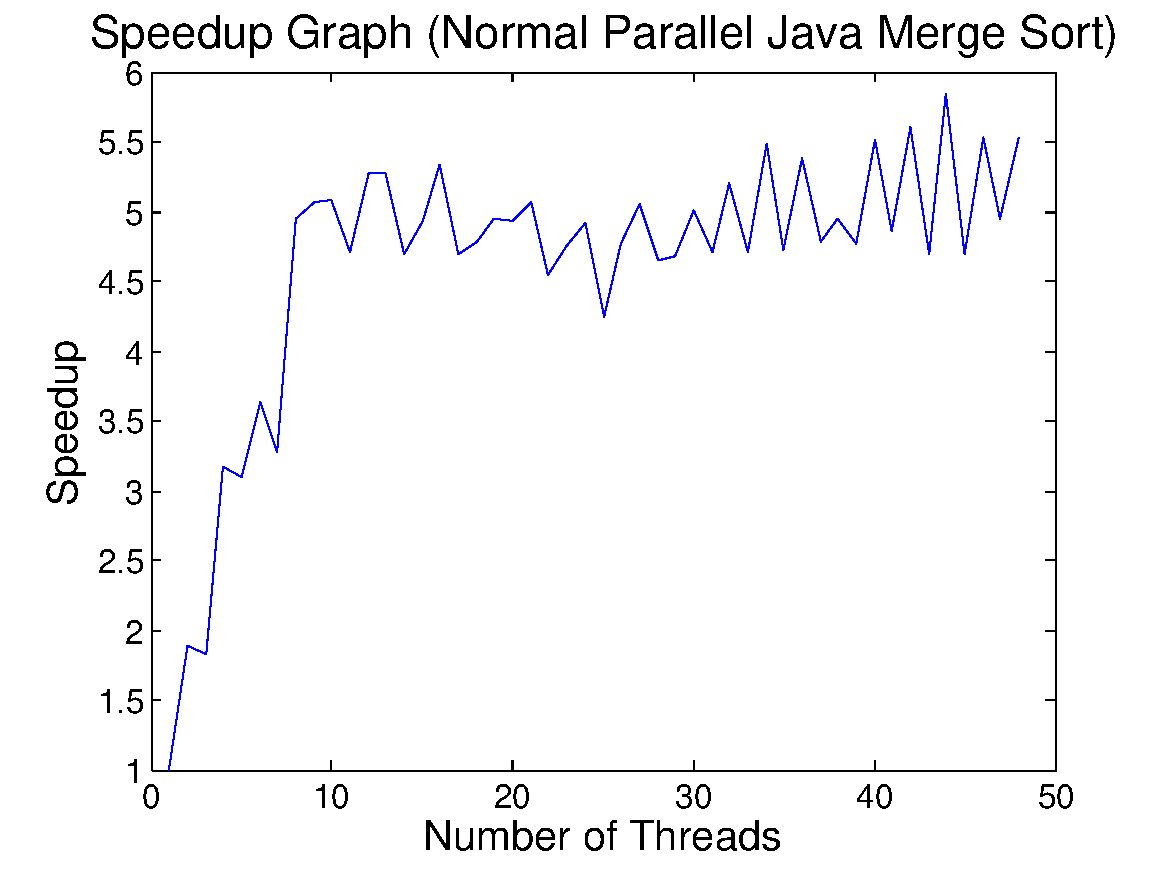
\includegraphics[width=\linewidth]{java_speedup_graph}
\caption[Parallel Java Merge Sort Speedup Graph]{The Java speedup graph, showing a merge sort written in Java, mirrors exactly what we have achieved by using the interface. The speedup in this graph plateau's at approximately 5 -- 5.5 which slightly greater than the
interface's merge sort results as would be expected since the interface constructed on a few layers and therefore will omit more overheads. This graph also includes a little jitter which is again due to the changes between the array's
values in between each test.}
\label{fig:java_speedup_graph}
\end{figure}
This is a very good sign to suggest that the interface is performing well. The normal Java merge sort reaches a peak speedup of around 5 whereas the interface provides a peak speedup between 3 and 4 which is a confident result for
both the OCaml-Java compiler and the interface. 

\subsubsection{Thread Scheduling Overhead}
The last section dealt with understanding the speedup properties of the merge sort algorithm and comparing that to the test results achieved. One important aspect that wasn't taken into account is the overhead caused by the scheduler
and how much that actually effects the computation time of the merge sort algorithm. We can determine the threading overheads in terms of the execution time of the merge sort by alternating the linear sort limit of the merge sort
algorithm -- which is the maximum array size that will be sorted on one thread, i.e. linearly. For a smaller linear sort limit, the merge sort algorithm does less computation per core and more lightweight threads are created as there
are more divisions of the array to be made before the linear sort limit is reached. However at some point we expect the lightweight threads to be sorting significant portions of the array such that the threading overheads are
negligible. Increasing the linear sort limit again beyond this point will result in a longer execution time as the algorithm will not divide the data up enough to keep all worker threads continuously busy. It is the point at which the
lightweight thread overheads become equal to the work done by the linear sorts which is important to us. At this point we can divide the execution cost roughly between thread scheduling and linear sort execution times in order to
calculate the average overhead per thread. The point at which this occurs is roughly the of the point at which the speedup gains from increasing the linear sort length begin to plateau. Figure~\ref{fig:sort_limit_graph} shows the test
results collected from increasing the sort limit along the x~axis for an array size of 30 million.

\begin{figure}[h!]
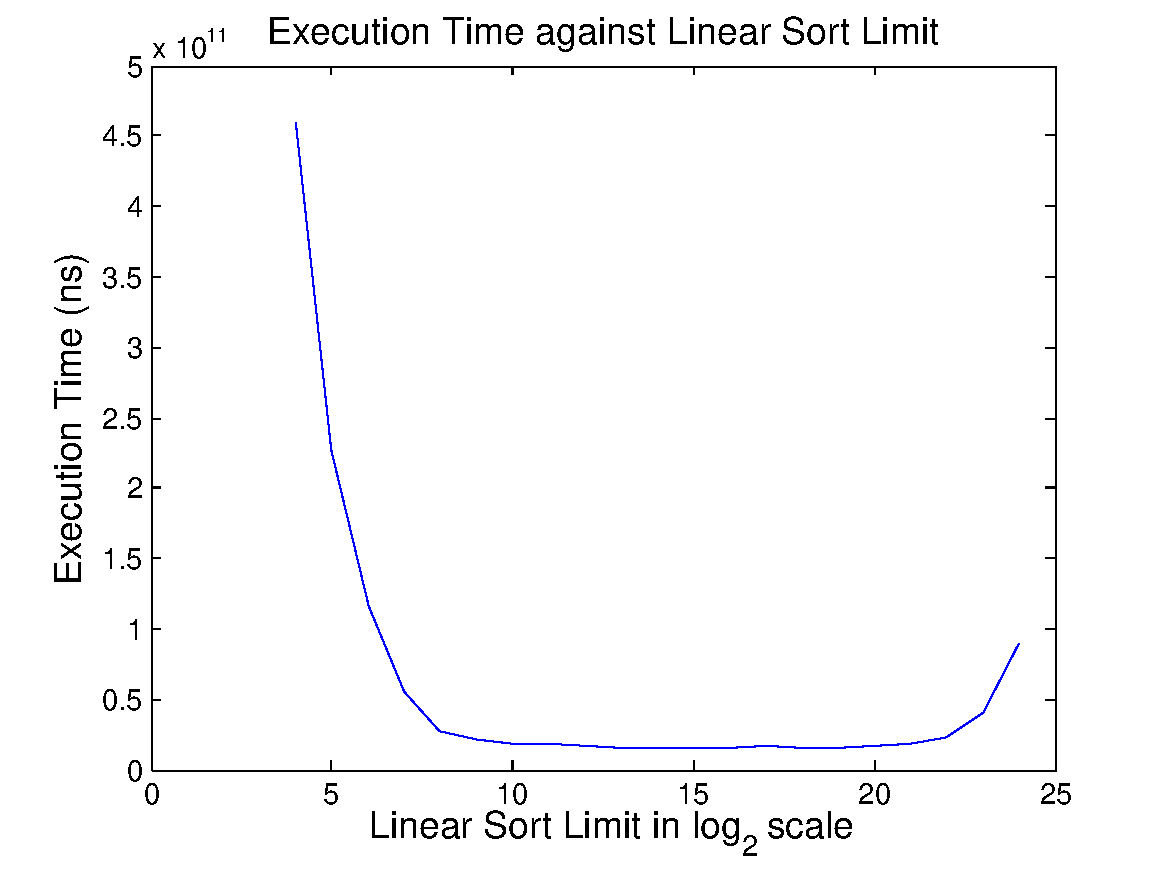
\includegraphics[width=\linewidth]{sort_limit_graph}
\caption[Merge Sort Linear Sort Limit Graph]{Sort limit graph showing the logarithmic increase in the linear sort limit on the x~axis along with it's effect on execution time on the y~axis. There is a steady decrease in execution time as the sort limit increases between
16 and 256, (4 and 8 on the x~axis). After this point the execution time seems to plateau until $2^{22}$ linear sort limit at which point the execution time begins to rise again. The initial decline is caused by the worker threads
performing more processing per thread which decreases the execution time. At the point of the plateau, the amount of work done by each thread is significant enough to keep all cores busy and the threading overheads negligible,
therefore we do not see any change in the execution time. The final rise at the right of the graph occurs as the sort limit tends towards the size of the array, so in fact the array is not being divided up enough to keep all the cores
busy.}
\label{fig:sort_limit_graph}
\end{figure}

It's clear to see the beginning of the plateau occurs around 8 on the x~axis, which being a $log_{2}$ scale corresponds to a sort limit of 256 values. The total amount of threads created at this point can be calculated as:

\[ threads = \lceil2^{log_{2}(30,000,000) - log_{2}(256)}\rceil - 1\]

Since the height of the merge sort array division tree is $\lceil log_{2}(30,000,000) - log_{2}(256)\rceil = h$ and the number of threads equals the number of leaves within the tree, calculated as $2^{h}-1$. Finally we simply need to
divide half the execution time by the total amount of threads to get the average overhead per thread in nano seconds:

\begin{align*}
avg\,overhead &= \frac{13426901208}{\lceil2^{log_{2}(30,000,000) - log_{2}(256)}\rceil - 1} \\
                    &= 0.11\,ms
\end{align*}

That's quite a long overhead for a lightweight thread, however considering that OCaml-Java itself is approximately 3 times slower in executing natively compiled OCaml code\cite{web:clerc2013} the large overhead was to be expected.
There are subtle ways to improve the overheads without interfering with OCaml-Java, however the speedup results of the parallel merge sort algorithm still show very positive results regardless of this thread overhead.

\section{Fibonacci}
\label{sec:fibonacci}
%
% Talk about Fibonacci in more detail. What it is, why it can be parallelised, etc
%
Also mentioned in section~\ref{sec:profiling} was the recursive Fibonacci algorithm for use in profiling the interface. The recursive algorithm is easily made parallel by spawning child threads at each recursive call until the base
case is reached. Each thread spawned is placed onto the yield queue, until a worker thread is able to pick it up and either perform the base case calculation or process the next recursive step -- creating more threads on the yield
queue. The parent thread will then synchronise on both child threads completing and use those results to calculate it's own Fibonacci result. This propagates back up the Fibonacci recursive tree until the final result is calculated
and returned to the initial caller function. The Fibonacci code used can be found in appendix~\ref{chap:code_samples} 

\subsection{Performance Analysis}
%
% Fibonacci didn't show good parallelism, graph shown in fig whatever.
%
\subsubsection{Execution Time}
The results of performance testing the recursive parallel Fibonacci algorithm are displayed in figure~\ref{fig:fib_time_graph}.
\begin{figure}[h!]
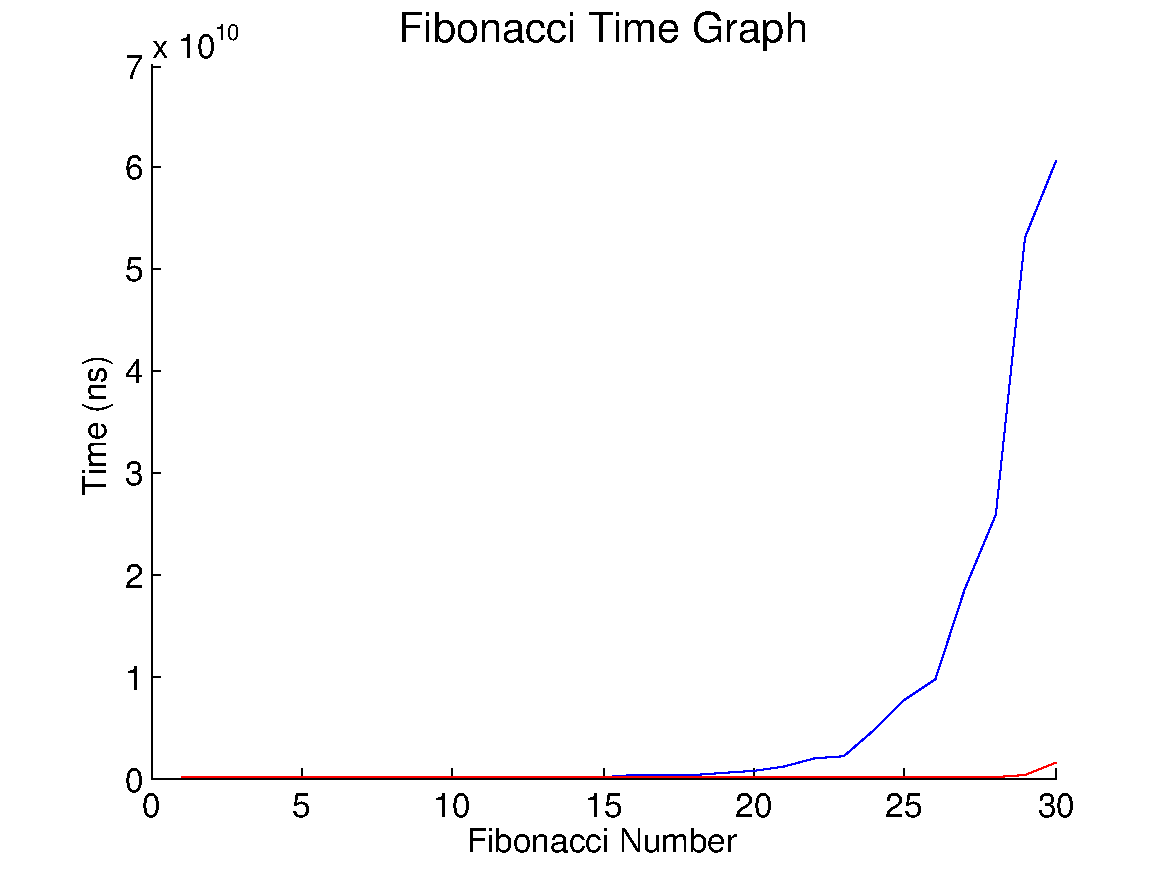
\includegraphics[width=\linewidth]{fib_time_graph}
\caption[Fibonacci Execution Time Graph]{The steeply rising line represents the parallel Fibonacci algorithm whereas the shallow line represents the single threaded Fibonacci algorithm. It is clear from this graph that despite having many cores available, the
threading overheads entirely overshadow the potential for speedup.}
\label{fig:fib_time_graph}
\end{figure}
This graph describes the execution time of the Fibonacci algorithm where the x~axis denotes the Fibonacci number being calculated and the y~axis denotes the time taken to calculate that Fibonacci number. The graph clearly shows that
calculating Fibonacci on multiple cores actually performs worse than using the same recursive algorithm on a single core. This is highly counter intuitive under the assumption that more cores means more power. Although there are many
more cores executing the Fibonacci calculations, it would seem the overhead of managing many LWT threads is significant enough to completely negate any potential speedup gains from utilising multiple cores.

%
% Why? Well its because fib does only an addition operation, therefore most of the processing goes into thread management overheads. made even worse since threads are small and made frequently (although actually I think it's made the
% same in this case)
%
At each stage in the Fibonacci calculation, a new thread is created for that recursive step. Once the thread is created, it is popped onto the yield queue and may sit there for a while until it is acquired by a worker thread to
perform execution. Within the calculation, the fib thread must bind on the result of both it's child threads and perform an addition. This bind operation consists of creating a closure containing an addition operation and the two
child threads, such that when they both complete, the closure will be called with their return values and pass the result back up the chain. We discovered in the last section that the average running time for all these steps is
roughly 0.11 ms which is a relatively significant amount of time. Furthermore all these extra steps are produced to simply perform a single addition operation which means the majority of the processing done on the worker thread is the
thread management rather than the algorithm processing.

% \subsubsection{Speedup}
% \todo{May remove this graph as I can't explain why more cores is worse even if parallelism isn't exploited, it should at least be the same...}
% The speedup graph also shows poor results using the current interface scheduling technique, which is shown in figure~\ref{fig:fib_speedup_graph}.
% \begin{figure}[h!]
% \includegraphics[width=\linewidth]{fib_speedup_graph}
% \caption{insert caption here}
% \label{fig:fib_speedup_graph}
% \end{figure}
% Almost resembling the merge sort speedup graph in figure~\ref{fig:msort_speedup_graph} upside down, the graph displays a negative speedup correlation against an increasing number of cores used to perform the calculation. This is a
% particularly strange result since you would expect that the execution time would at least be roughly the same given that you are adding more processing power. However clearly there must be some externalities in play, similar to the
% scheduler overheads from the previous section. 
% 
% The most sensible explanation of the results seems to be lock contention which the Fibonacci calculation exposes
% might just remove this graph
%The graph in figure blabla\todo{insert fib speedup graph} shows the relative speedup of calculating the value $fib(30)$ on a linearly increasing amount of cores, given by the x~axis. The data demonstrates a steep decline within
%the first two cores becoming enabled and then a steady and far more shallow decline beyond this point. Again a similar problem to that previously demontr

%
% Some sort of discussion section should go in here?
%

%
% Possible ways of improving the result is to reduce the threading overhead somehow, perhaps by assigning processors to subtrees of the Fibonacci calculation until every processor is in use, then allow them to calculate the rest of
% the sub tree. That would involve using a different scheduling technique which was of course part of my extended options if time allowed.
%
Overall the Fibonacci calculation has not scaled well with the current implementation of the interface, unlike the merge sort. However it may be possible to achieve better performance gains by using a different scheduling technique
than the one currently in use. Furthermore the current implementation of the parallel Fibonacci continues to recurse until it reaches $fib(0)$ or $fib(1)$, by limiting the recursion depth of the Fibonacci algorithm in a similar
fashion to the linear sort limit of the merge sort algorithm, we can combine more processing potential into a single lightweight thread and definitely achieve better results.

\section{Summary}
Within this chapter, I discussed how the merge sort algorithm was tested and also the performance of the merge sort algorithm when executed with the interface. The results obtained demonstrated the interface's true ability to utilise
multiple cores and execute parallel LWT code with appropriate speedup gains, achieving a speedup of 3 -- 4 in comparison to a normal Java merge sort algorithm which achieved a speedup of 5 -- 5.5 with the same test parameters. The
reason to the graph shape was proven as the theoretical speedup of the merge sort algorithm and was observed in both the interface parallel merge sort and the normal Java merge sort results. We also used the variation of the linear
sort limit to determine the approximate thread management overhead of the lightweight threads, which resulted in 0.11 ms -- a good result considering OCaml-Java's approximately 33\% reduction in execution speed.

The parallel Fibonacci algorithm provided somewhat different results as we discovered the recursive Fibonacci algorithm mainly exposed thread overhead times since the algorithm continues to recurse until it reaches $fib(0)$ or
$fib(1)$. However we determined that setting a recursion limit would move the majority of the processing time from thread management to algorithm execution in a similar way to the linear sort limit in the merge sort algorithm.

\chapter{Conclusions}
\label{chap:conclusions}
% Talk about what I wanted to do with the private public threads, how that would've overcome the `half-baked' threads problem and allowed me to construct a workstealer. The contention on the single thread queue could've been
% aleviated.
% talk about how I took on a massive project but should've broken it down to make it easier on myself.
%
% Overview of this chapter
%

%
% Achievements and what I would've liked to continue working on
%
\section{Lessons Learnt}
The final result of my dissertation has been successful. I have managed to complete all my success criteria and produce an interface which scales similarly to natively written Java code when comparing popular parallel benchmarks such as merge sort. Admittedly taking on such a
large OCaml code base with only little prior knowledge of ML was a feat I under anticipated. The languages have a few differences, however the styles of development in the two languages are very independent of each other. A lot of the
focus in learning ML was put on developing algorithms and data structures, whereas OCaml's Core library contains most of these algorithms and has an emphasis on using them instead. Furthermore in languages like C++ and Java there are
structured and tested ways of producing systems with low coupling and high cohesion via object oriented programming techniques and design patterns, however in OCaml you can choose to use the modular system, the object system, neither
or a mixture of both\cite{chailloux2000}. 

That being said, I've learnt a lot of important lessons about developing functional code and also project management. One of the main problems I had with this project was biting off more than I could chew. At times within LWT there
was very high coupling between modules and I found myself attempting to juggle developing and converting code from many different locations in code at the same time in an attempt to keep the entire system working. Inevitably it served
me better to attempt to reduce coupling as much as possible and focus on core sections of the code base, rather than as a whole. At times it was also characteristic of me to become `lost in the code', where I would be thinking of many
other things I could do to better my project or produce cleaner code/tests. Whilst this is perhaps a good mindset to have when dealing with a project it can at times lead me astray from my targets and success criteria, therefore it
was good to take a minute, step back and look at the picture as a whole: where I am right now, where I need to be and what I need to do to get there.

\section{Future Work}
In conjunction to the work already demonstrated within this project, I also have some ideas on how else some of the challenges in this project could have been overcome -- it would be interesting to see how the performance changes
depending on how the interface is implemented.

\subsection{Public/Private Queues}
In section~\ref{subsubsec:thread_safety} I mentioned the `Half-Baked Thread' problem which meant that useless yield threads were being placed onto the yield queue and immediately removed by other threads before having any useful
bindings attached. One other solution to this problem I have thought about was to have a separate private and public queue per worker thread. As a worker thread is executing some code within an LWT thread, it will place any created
threads into its private queue, which may contain threads that are or are not able to be executed. No other worker thread may have access to the private queue of any other worker thread. Once an LWT thread has terminated, the private
queue will contain the new spawned threads which resulted from the LWT threads execution, furthermore they will be in a state where they are all ready to execute. The worker thread must then move these ready threads to the public
queue, all bar one, and begin execution of the one retained thread. By keeping all the threads in the private queue until the LWT thread has finished execution, there is no chance that another thread will come along and take the
incomplete thread and begin executing it. Only threads on the public queue are able to be taken by other threads for execution.

\bibliography{resources}

\appendix
\chapter{Notes}
\section{Machine Specifications}
\label{apdx:machine_specifications}
The following are specifications for the machines used during the testing and development of the interface:

\subsubsection{`Roo' Multi-core Machine - Main Test Machine}
\begin{itemize}
\item {\em Processor} \hfill \\
AMD Opteron\texttrademark\ 6344 Processor (12 logical cores, 6 physical cores @ 2.6 GHz) ($\times4$)
\item {\em Main Memory} \hfill \\
64GB RAM
\end{itemize}

\subsection{Macbook Air 2013 - Main Development Machine}
\begin{itemize}
\item {\em Processor} \hfill \\
Intel Core i7 (4 logical cores, 2 physical cores @ 2.6 GHz)
\item {\em Main Memory} \hfill \\
8GB RAM
\end{itemize}

\chapter{Code Samples}
\label{chap:code_samples}
The following appendix contains relevant code samples which have been referred to within my dissertation.

\section{Recursive Parallel Fibonacci Implementation (fib.ml)}
The recursive Fibonacci algorithm was implemented 3 times in different ways in order to compare the normal, asynchronous and parallel versions for execution time, speedup and other relevant measurements. The following code listing
shows each of these versions.
\lstinputlisting[frame=none]{fib.ml}

\section{Parallel Merge Sort Implementation (msort.ml)}
Similar to the Fibonacci implementation, the merge sort was also written in three different ways.
\lstinputlisting[frame=none]{msort.ml}

\section{Worker Thread}
The following code runs on each Java worker thread and processes lightweight threads until interrupted, this loop is relatively small in order to try and keep the bulk of the processing in the lightweight thread rather than the thread
management overheads.
\lstinputlisting[frame=none]{worker.ml}

\chapter{Project Proposal}
\label{chap:proposal}
\section{Introduction}
\label{sec:introduction}
The concept of functional programming is becoming far more widespread and important in recent times. Object orientated and imperative languages like C++ and Java are beginning to use functional concepts such as type inference, first-class functions and more. The C++11 specification defines a new `auto' type which causes the compiler to infer the variable type from its content\cite{web:autokeyword}. Furthermore, Java 1.8 now includes Lambda Expressions in conjunction with a range of modifications to the libraries that allow its use\cite{web:javalambda}. Companies such as Jane Street -- a quantitative trading firm -- use OCaml entirely for all their high performance trading software and algorithms\cite{web:janestreettech}, and contribute to the advancement of the OCaml language.

OCaml is a great example of a powerful and robust functional language. It includes everything you would expect from a functional language and more such as object orientated and imperative programming paradigms, and is derived from the highly expressive ML programming language. Its powerful type system provides great type safety, eliminating many of the associated runtime errors; automatic memory management through it's incremental garbage collector and strict evaluation branching from it's ML roots in theorem proving. Parallelism in OCaml is however limited due to a global runtime lock present in the system. The purpose of this lock is to prevent unsafe use of non re-entrant code within the core OCaml library, but more importantly is present due to the fact that the OCaml garbage collector is not multi-core friendly\cite{clerc2012}. The resulting issue is that only one piece of OCaml code may be executed at a time leading to very little capacity for parallelism.

Java on the other hand is a widely supported, widely available software platform and programming language used in devices like desktop/laptop PC's, mobile phones, ATM's and even credit/debit cards\cite{web:aboutjava}. Its huge community of developers, wide selection of libraries and ability to write easily portable and distributable software means it has continued to grow rapidly over the years. Java also has a thread safe concurrency library which works in conjunction with its parallel and concurrent G1 garbage collector.

Both languages have their pros and cons however the OCaml-Java project aims to bring the best of both languages together by compiling OCaml to Java bytecode, taking advantage of OCaml's powerful typing system and Java's feature rich library. In addition, OCaml code compiled with OCaml-Java uses Java's G1 garbage collector meaning that the software is able to run in parallel across multiple cores without restriction. OCaml-Java comes with a relatively low-level concurrency library which allows developers to utilise its multi-core capabilities, however these low-level modules can be cumbersome to use frequently, especially considering there are some very popular and powerful concurrency libraries for OCaml -- such as Ocsigen's Light Weight Threads (LWT).

\section{Substance and Structure of the Project}
\label{sec:substance}
The aim of this project is to port the LWT concurrency library to use OCaml-Java's low-level threading library therefore taking advantage of Java's multi-core processing capabilities and providing an easier, more robust means of writing parallelised OCaml code to run on the JVM. LWT is a widely used monadic concurrency library for OCaml with strong emphasis on the `light' aspect of their threads. Spawning a thread in LWT is a very cheap operation and as such, threading with LWT fits well with the short-lived-data aspect that is well acquainted with functional languages. Furthermore the results of the project will provide some interesting results into the increased scalability of OCaml code running in parallel across multiple cores.\\
Thinking modularly, the project can be divided into three distinct sections:
\begin{description}
\item[Porting the LWT Library:] Porting the library to use OCaml-Java will allow the execution of software written in LWT under OCaml-Java, running on a single thread. This will mainly consist of writing a back-end to act as a pipeline between LWT and OCaml-Java. 

\item[Making LWT parallel:] Making the ported LWT library parallel will mean utilising many Java threads to execute the LWT threads. These LWT threads are as mentioned very lightweight and are frequently spawned, Java threads on the other hand are not lightweight and as such a one-to-one mapping of LWT to Java threads will not be possible. To resolve this issue, and thus connect the two sides of the equation, an appropriate scheduler must be written to distribute LWT threads between the fewer Java threads that are active on each core.

\item[Benchmarking:] The final aspect of the project is to evaluate how the scalability of software written in LWT scales when run under my ported version as opposed to when run under default OCaml. It will be necessary to convert existing parallel processing benchmarks to use the ported LWT library and also test the scalability on hardware of varying parallel processing power, such as on a dual-core, quad-core and 48-core machine.
\end{description}

\section{Success Criteria}
\label{sec:success}
For the project to be a success I have set the following requirements:
\begin{enumerate}

\item{I am able to show the scalability difference between two programs using the same piece of LWT code, one compiled using the original LWT libraries under the normal OCaml compiler and one compiled using my ported LWT libraries under OCaml-Java, running on the JVM.}
\item{Parallel processing benchmark can be used to determine the scalability using LWT under OCaml-Java and using LWT under the normal OCaml environment.}
\end{enumerate}

\section{Starting Point}
\label{sec:starting}
My experience in functional programming extends as far as the ML courses in Part IA, however I enjoyed completing Project Euler challenges in ML (of which I was normally one of the few people to do so!). Neither have I developed code of a substantial size in ML or OCaml, therefore the best place place to begin would be looking into the structure of open source OCaml code and get a feel for how things are laid out in OCaml. In addition the book `Real World OCaml'\cite{madhavapeddy2013} has a public beta available before publication (lucky for me) which will also provide a solid foundation in producing real world OCaml code.

This project relies on the OCaml-Java project, an OCaml to Java bytecode compiler, developed by Xavier Clerc at INRIA. This project provides the ability to use the numerous Java libraries as well as Java's already mentioned parallel processing capabilities. Furthermore the JVM can be found installed on many different types of hardware and systems meaning the target hardware for OCaml code will be greatly increased by using OCaml-Java. Xavier Clerc, having strong connections with the OCaml Labs here in Cambridge, is also keen to support this project. The version of OCaml-Java I will be using is an early preview release of version 2.0.

Finally getting to grips with the innards of LWT will be most easily achievable by experimenting with the software first hand and diving into the source code available on Github.

\section{Optional Extensions}
\label{sec:optional}
Some ideas for optional extensions include:
\begin{itemize}
\item{Experiment with different schedulers to see which perform better and investigate why.}
\item{Attempt to get higher compatibility rate than initially decided which would mean ironing out incompatibilities with current software written with LWT when run with my ported libraries.}
\end{itemize}

\section{Timetable and Milestones}
\label{sec:timetable}

\begin{description}
\item[17$^{th}$ Oct -- 6$^{th}$ Nov] Further research into LWT's source. Research OCaml coding techniques.\\
Milestone: Complete LWT coding tutorial; Read through `Real World OCaml'; Implement some parallel programs in OCaml-Java 2.0; ready to begin planning.

\item[7$^{th}$ Nov -- 27$^{th}$ Nov]
Continued research into LWT's source. Plan implementation of basic functionality of the ported library.\\
Milestone: Ready to begin development.

\item[28$^{th}$ Nov -- 18$^{th}$ Dec] Begin porting LWT to single threaded interfacing with OCaml-Java.\\
Milestone: Some basic functionality implemented.

\item[19$^{th}$ Dec -- 8$^{th}$ Jan] Continued porting of LWT to single threaded interfacing with OCaml-Java.\\
Milestone: Porting complete. Should be able to walk through the LWT tutorial without much/any hassle.

\item[9$^{th}$ Jan -- 29$^{th}$ Jan] Begin creating the scheduler to manage the distribution of LWT threads to OCaml-Java threads.\\
Milestone: Fixed number of Java threads are able to be scheduled to, regardless of number of cores on system.

\item[30$^{th}$ Jan -- 19$^{th}$ Feb] Continued scheduler development.\\
Milestone: Number of Java threads scales with the number of cores present on the system.

\item[20$^{th}$ Feb -- 12$^{th}$ Mar] Begin conversion of parallel processing benchmarks.\\
Milestone: Most of benchmarking software conversion complete, fixed relevant bugs which may arise from testing with the benchmark.

\item[13$^{th}$ Mar -- 2$^{nd}$ April] Testing with benchmarks, finishing dissertation evaluation and write-up.\\
Milestone: Relevant scalability graph data accumulated.

\item[3$^{rd}$ April -- 23$^{rd}$ April] Finalising dissertation write-up.\\
Milestone: Dissertation complete!

\end{description}

\section{Resources Required and Backup}
\label{sec:resources}
A list of required resources:
\begin{itemize}
\item{My own Machines:
    \begin{itemize}
    \item{Macbook Air 13" 2013 (8GB RAM, 512GB Storage, OSX/Windows 8)}
    \item{Desktop Computer (Ubuntu 13.04/Windows 7, Intel Core2 Quad, 5TB Storage)}
    \end{itemize}
}
\item{Machines in College}
\item{A many-core machine in the SRG (32 - 48 Cores; e.g. `Roo')}
\item{OCaml-Java and Sources\footnote{OCaml-Java: http://ocamljava.x9c.fr/}}
\item{OCaml\footnote{OCaml: http://ocaml.org}}
\item{LWT Sources\footnote{LWT: http://ocsigen.org/lwt/}}
\end{itemize}

Backups will be provided by Dropbox, Skydrive, my own personal USB stick and my personal storage on the PWF facilities. Cloud backup will be incredibly useful for keeping my data accessible from many locations and also avoiding local corruption which could occur at any time.
Version control (and also the main copy of my dissertation/project) will be provided by Github. I chose Github since I am already very familiar with git version control; Github provides cloud storage so I'm able to retrieve and work on my files from various locations; furthermore Github provides free private repositories for students.




\end{document}
